%% LyX 2.0.3 created this file.  For more info, see http://www.lyx.org/.
%% Do not edit unless you really know what you are doing.
\documentclass[CJKchapter,noabcount]{CAS}
\usepackage[utf8]{inputenc}
\setcounter{secnumdepth}{3}
\synctex=-1
\usepackage{color}
\usepackage{bm}
\usepackage{array}
\usepackage{longtable}
\usepackage{textcomp}
\usepackage{amssymb}
\usepackage{mathrsfs}
\usepackage{makeidx}
\makeindex
\PassOptionsToPackage{normalem}{ulem}
\usepackage{ulem}
\usepackage{nomencl}
%\usepackage[numbers,sort&compress]{natbib} 
\usepackage{hypernat} 
% the following is useful when we have the old nomencl.sty package
\providecommand{\printnomenclature}{\printglossary}
\providecommand{\makenomenclature}{\makeglossary}
\makenomenclature
\usepackage[unicode=true,pdfusetitle,bookmarks=true,bookmarksnumbered=true,bookmarksopen=true,bookmarksopenlevel=2,
 breaklinks=false,pdfborder={0 0 0},backref=false,colorlinks=false] {hyperref}

\makeatletter

%%%%%%%%%%%%%%%%%%%%%%%%%%%%%% LyX specific LaTeX commands.
\providecommand{\LyX}{\texorpdfstring%
  {L\kern-.1667em\lower.25em\hbox{Y}\kern-.125emX\@}
  {LyX}}
%% Because html converters don't know tabularnewline
\providecommand{\tabularnewline}{\\}

%%%%%%%%%%%%%%%%%%%%%%%%%%%%%% User specified LaTeX commands.
\usepackage{tikz}
\usepackage{pgfplots}
\def\oc{\ensuremath{^\circ\hspace{-0.09em}\mathrm{C}}}
%\usepackage{CJKfntef}format=hang 
%\captionsetup[figure]{justification=centering,singlelinecheck=false}
%\captionsetup[figure]{format=hang}
%\usepackage{xstring}
%\raggedbottom

\@ifundefined{showcaptionsetup}{}{%
 \PassOptionsToPackage{caption=false}{subfig}}
\usepackage{subfig}
\makeatother

\begin{document}

\confidential{}


\title{Global observation of PKiKP and its coda, implying heterogeneous\\ %
structure of the inner core}


%\subtitle{——基于Xe\LaTeX{}、\LyX{}与JabRef}


\author{龙鑫}


\thesistype{硕士学位论文}


\tutor{艾印双\quad{}研究员}


%\tutorinstitute{中国科学院地质与地球物理研究所}


\institute{中国科学院地质与地球物理研究所}


\degree{理学硕士}


\major{固体地球物理学}


\date{2016年6月}


\etitle{\uline{Global observation of PKiKP and its coda, implying heterogeneous
structure of the inner core}}


%\esubtitle{\uline{---Case studies of elevated soil warming}}


\eauthor{Long Xin}


\etutor{Ai Yinshuang}


\emajor{Solid Geophysics}


\edegree{Master}


\emajortype{Science}


\einstitute{Institute of Geology and Geophysics\\
 Chinese Academy of Sciences }


\edate{June, 2016}

\maketitle

\Declaration{关于学位论文使用权声明}

\frontmatter

\begin{abstract}
从实际的稠密台阵中抽取各种几何形态和台间距不同的子台阵,运用PWS等标准台阵叠加技术,比较不同类型的子台阵对与内核相关的一系列弱震相(如前临界PKiKP、PKIIKP和PKJKP等)提取的效果;然后通过理论模拟各种不同台阵的情形,进行叠加,将理论模拟的最佳结果和使用实际资料叠加的结果进行比较。若能找到最优的配置方法,则对今后以关测与内核相关的弱相位为目的的地震台阵布设具有一定的指导作用。
\end{abstract}

\keywords{台阵;叠加;PWS;弱震相;内核}

\begin{eabstract}
 I collect global data set from short period IMS arrays, from which waveform quality of each station is relatively high and records last several decades for their nuclear detection purpose, and Hi-net which is extremely dense. I attempt to use those data and apply array stacking technique like PWS to detect and identify the inner core relevant weak phases. I also plan to figure out a best array configuration for the signal extraction, which is mainly affected by geometrical distribution of stations and slowness of a given phase using real data and theoretical stimulation, and consider to determine a proper array size that would be sufficient to provide a good SNR for the phase extraction. The result of this research would be a guidance for future devise of seismic array aimed to study the inner core properties using weak inner core phases.
\end{eabstract}

\ekeywords{Array;Stack;PWS;Weak Phases;Inner Core}

\tableofcontents{}

\mainmatter

%\chapter{引言}

\section{CMB的小尺度变化}

地球的核幔边界(CMB)在地球内部的动力学演化过程中具有非常关键的作用,由于它和地幔、地核的对流有
着紧密的联系,对其性质的了解有助于我们认识地球的演化. 许多地震学的研究揭示了这个界面存在复杂的性质并
伴有强烈的区域性变化. 

在这些可能存在的复杂结构中,超低速带(ULVZ)常常受到关注. 它的典型特征是具有低的P和S波波速,并较周围结
构有更高的密度,前人的研究发现这种结构常常存在于大剪切波低速省的附近~\citep{Garnero2008}. ULVZ通
常被认为尺度很小(约数百千米),因此也较难用层析成像等地震学手段探测到. 之前的研究常基于异常大的PKP前驱波~\citep{vidale1998evidence,Thomas2009}或者异常的SKP${}_{diff}$S走时延迟~\citep{Thorne2004a,Garnero1995}来推断ULVZ的存在,在一些研究中,短周期的PcP和ScP被
用来提高对CMB结构探测的分辨率~\citep{Castle2000,Rost2004a}. ULVZ的存在可能造成PcP的复杂特性,
当低速带与其上部地幔有较大速度差的情况下,PcP主震相前将出现由ULVZ顶部反射的前驱波,其后可能出现P到S
波的转换震相,并且由于反射系数的减小,PcP的振幅也会显著降低~\citep{Gassner2015}. 目前多数研究认为这种低速结构的形成可能是源于CMB上部物质的部分熔融,比如含水的洋中脊玄武岩(MORB)下沉到地幔底部,降低了周围物质的熔点而产生熔融,而且这些MORB受到地幔对流的影响更易于集中在化学性质差异明显的边界比如LLSVPs的周围~\citep{Xu2009a}. 除此之外还有一些其他的机制用来解释其成因,有实验模拟研究认为这种低速结构来源于地幔于外核物质的化学反应~\citep{Hirose2005a},或者CMB底部的物质沉积~\citep{Buffett2000a}. \citet{He2006a,He2012a}通过ScS-S、ScS2-SS走时残差和波形模拟尝试确定了太平洋低速异常的边界,并认为太平洋边界底部的ULVZ从异常内延伸到周围的高速区,并且这种扩张在小尺度内存在强烈变化,这暗示了太平洋异常低速异常可能存在变化的物质组成以及同周围地幔物质复杂的接触关系. 

CMB另一个重要的特征是它的界面起伏,根据之前的研究结果,其横向尺度可能从数百至数千千米;深度变化从几
百米至数百千米~\citep{Earle1997,Sze200327}. CMB的界面起伏会强烈影响PcP的观测,一个局部上凸的界面会造成波场
能量的发散,因此减小PcP的振幅,而一个局部下陷的CMB界面会产生相反的效果,即造成能量的汇聚,从而增大PcP的振幅~\citep{Kampfmann1989a,Neuberg1991}. \citet{Rost2004a}利用Yellow Knife台阵观测
到异常大的PcP振幅,并结合P作为参考震相进行分析,认为在阿拉斯加的Kenai半岛下方的CMB上存在局部的下凹. 最近,\cite{Wu2014a}利用表示定理模拟了不同横向尺度和深度变化参数组合的CMB起伏下的PcP
波形,结合之前在Kenai半岛下方CMB反射的PcP数据,检验了CMB界面起伏对PcP的影响. 其结果显示,一个下陷6千米,横
向宽度6{\textdegree}的界面起伏会造成PcP振幅放大4.5倍. 但是,在P波衰减和PcP振幅增大之间仍然存在一
个折衷效应,因为之前的研究通常使用P作为参考震相,而在上地幔中,直达P波和PcP的传播路径存在很大差异,且
P波的射线参数较大,受到横向变化的影响也更大. 如果在上地幔或者在台站下方的沉积层经历到强烈衰减,之前研究
所估计的CMB对PcP振幅放大效应可能就不那么显著了,因此界面起伏的尺度也可能被错误估计. 假设,在小尺
度下,ICB的性质是稳定的,而且没有大的起伏变化,引入PKiKP将其作为一个新的参考震相可以改进对CMB结构的
约束. 因为在震中距不大的情况下(30{\textdegree})PKiKP和PcP离源角相差一般不到10度,在上地幔的传
播路径比较接近并且外核可被认为是均匀的~\citep{Stevenson01011987},所以来自上地幔的干扰和震源辐射花样差异的影响都将尽可能减小. 

\begin{figure}
\centering
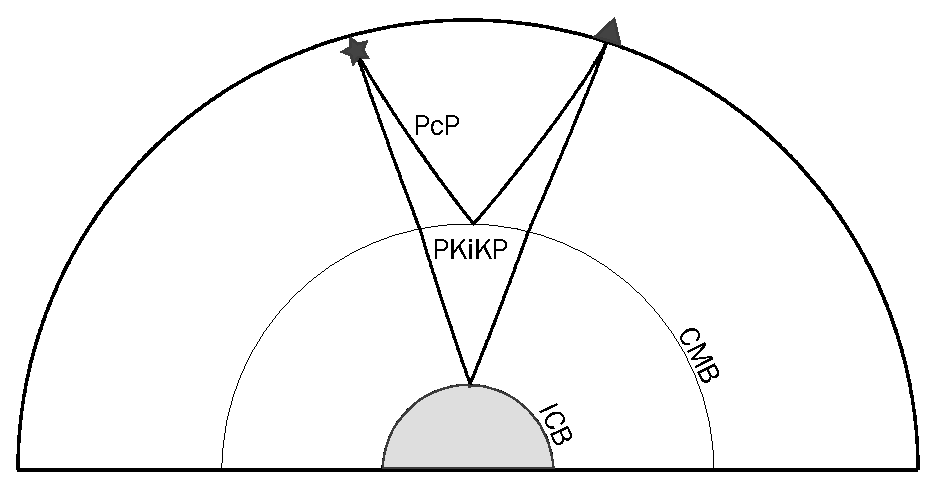
\includegraphics[width=0.7\linewidth]{fig/chap1/ray_path}
\caption{PcP和PKiKP射线路径示意图}
\label{fig:ray_path}
\end{figure}

\section{PKiKP/PcP振幅比的强烈离散}
作为内核冷凝增长和内核与外核相互作用的场所~\citep{Deguen2011,Bergman2010},地球的内外核边界(ICB)的物理性质一直也是地震学的重要问题之一. 到目前为止,对ICB的研究基本都是利用由该界面反射的PKiKP震相,而PKiKP也是内核存在最为直接的证据. PKiKP又分为前临界和后临界,在早期的观测条件下,后临界PKiKP(又被成为PKP${}_{df}$)的观测要更为容易,其作为参考震相,通常与PKP${}_{bc}$结合,被用于研究内
核顶部的结构~\citep{Tanaka1997}. 相比而言,由于较小的反射系数和较低的信噪比,加上观测条件的限制,
在早期对于小震中距情况下的前临界PKiKP的观测数量非常有限~\citep{Bolt1970},但还是有研究尝试利用PKiKP/PcP振幅比来估计内核的密度和ICB波速跃变~\citep{Souriau1989,Shearer1990}. 由于PcP和PKiKP在浅部结构中传播路径的相似性(图\ref{fig:ray_path}),这种使用振幅比的
方法假设可以消除地幔结构、台站响应等因素对观测结果的影响而且CMB是平坦且横向变化不大的,观测到振幅比异
常则来自内核,由此估计ICB的物理参数. \citet{Krasnoshchekov2005}用记录到核爆事件产生的PKiKP绝
对振幅来约束ICB的区域变化,推测出内核表面存在马赛克结构. 虽然振幅经过了震级校正,但台站的增益及场地效
应依然是不确定的因素. 因此,关于ICB的研究大多使用PcP作为参考震相. 随着近年来大规模地震台阵的安装和区
域性密集台网的布设,PKiKP的观测数量显著提升,通过搜索全球1995至2000年的IMS小口径台阵数据,利用叠加方法,\citet{Koper2004a}搜集了三百多个PKiKP观测,远远超过之前的观测数量的总和;利用Hi-net,\citet{Kawakatsu2006}首次报道了由一个地震产生的超过100个清晰的PKiKP记录,通过慢度分析和波形拟合,有
力地证实了尖锐ICB的存在. 虽然PKiKP的观测数量大大提升,但用它和PcP约束内核参数仍然面临很多困难. 首先
在小震中距情况下,PcP容易被S波的尾波干扰,因此限制了可用的数据量;其次,由于台阵口径有限,PKiKP在内核的反射有限,很难将所有采样区域的观测结果联系起来并结合地球动力学机制进行讨论~\citep{Tanaka2015a};再次,即使在很小的区域,观测到的振幅比也可能呈现出非常离散~\citep{Koper2004a},但造成数据离散
的来源却很难确定. 

大量观测表明内核并不是一个物性均一的刚性球体,除了波速的各向异性~\citep{Wang2015},现在也已有较多的
观测证据支持内核内部的不均匀性结构,像1-degree的东西半球的速度和衰减的不均匀~\citep{Tanaka1997,Wen2002}和内核顶部局部的小尺度散射结构~\citep{Vidale2000a}等. 一些地球动力学模型试图对这些结构的成因给出解释,如既有外核大尺度的非对称流~\citep{Aubert2008,Gubbins2011},也有来
自内核自身的内部对流~\citep{Alboussiere2010,Monnereau2010},但还没有一种模式能完全解释地震观
测. ICB是连接内外核的桥梁,因此可能对内核结构作出一定反映,因而一些最近的研究尝试将全球的PKiKP/PcP
振幅比和走时分布与内核的东西半球差异这种模式联系起来,但由于全球数据的离散,这种尝试看上去并不可行~\citep{Waszek2015a}. 

PKiKP/PcP振幅比和走时残差的区域性离散可能有多种来源. 其一,尽管PcP和PKiKP的离源
角相差不大,它们在的传播路径还是有一定差异,因此在地壳和地幔中的所经历的衰减和不均匀性结构也会有所不同,
从而贡献振幅比和走时差的异常~\citep{Tkalcic2010a};其二,由于PKiKP射线较PcP更陡,其受到横向结构
变化的影响较小,尤其是二者受震源附近和近台站下方的结构影响的差异;其三,也是本研究关注的主要内容,如前
面所述,CMB结构会不仅会造成PcP振幅的剧烈变化,其走时也会受到影响~\citep{Koper2003}. 然而,CMB对观
测的影响却很少被之前很多研究所提及或仅有少许讨论~\citep{Cao2004,Waszek2015a,Dai2012,Tanaka2015a}. 即使注意到了可能的CMB效应,使用之前的分析方法也很难将造成数据离散的来源确定~\citep{Koper2004a}. 除了以上因素,台站的信噪比条件同样不能忽视,因为PcP和PKiKP的到时不同,而两者被记录时的信噪比
环境也不相同. 综合上面的考虑,如果不能将每种来源小心地区分出来,用振幅比和走时残差的方法就很难得到真实
的ICB物理参数的估计. 

\section{本研究的主要工作}
由于短周期PcP(1--2Hz)对CMB结构变化敏感,能提供对该界面性质最直接的约束,且PKiKP 和PcP的振幅比呈现强烈离散,而异常可能源于CMB结构对PcP的影响,这就使得可以通过振幅比的变化推测CMB结构变化. 另外,以PKiKP作为参考震相,不仅可以减小由浅部结构产生的不确定性还可以有效判断引起PcP波形变化的来源. 因而利用PcP和PKiKP研究CMB结构变化存在很好的可行性,

本硕士论文的主要工作是首先通过收集全球IMS(International Miscellaneous Stations)小口径台阵记录到的PcP和PKiKP数据,从中筛选出产生同时被两个邻近小口径台阵记录到PKiKP和PcP信号的地震事件,这两个台阵的震中距也相近,通过对比两个台阵的观测包括PKiKP
和PcP的振幅比、走时残差和波形来确定产生区域性离散的PKiKP/PcP振幅比的来源;当没有两个相近震中距的相
邻台阵的时候,通过分析多个相邻地震产生的被同一台阵记录到的PKiKP和PcP信号,并结合前人的研究结果,来推
断观测异常的成因. 利用IMS小口径台阵,不仅可以提高观测的可靠性,得出对于某个台阵的平均振幅比,以此有效
评估台阵观测的可信度,而且经过对不同台阵、地震事件和震相的比较后,一些可能对观测造成影响的因素可以被排
除,并且确认CMB的界面起伏变化和低速结构可以基本上解释PKiKP/PcP振幅比在小尺度范围内的强烈离散以及PcP的
变化. 虽然研究使用的还是常规的走时和振幅分析方法,但通过运用以上对比方法,有效地改善了对CMB小尺度结构
的分辨能力. 除了IMS小口径台阵的观测,本研究还补充了国家测震台网的数据,利用大规模的采样来分析大尺度范围内的CMB结构变化. 为了评价单台站的观测结果和分析不确定性的来源,本研究还对重复地震的PKiKP和PcP数据进行了分析和比较. 最后,尝试将本研究的观测结果和之前的地球动力学模拟结合起来,简要讨论CMB各种变化的形成机制. 

%\chapter{原理与方法}

引言中提到的与内核相关的弱震相在实际资料中都十分稀少,但它们对内核物理性质的研究却非常重要,
就目前来说甚至是不能被其他方法所替代的,如自由震荡\citep{DZIEWONSKI1971};存在分辨率不高
的缺陷;目前比较流行的噪声干涉方法最初用于提取地球表层面波信号\citep{Snieder2004}, 最近
也有关于内核相关的体波提取的发现\citep{Lin2013,Lin2013b}, 但都还处于初步的研究阶段。所以
相比而言,较为“传统”的地震台阵方法对于这些内核弱震相的提取还是很重要的。

地震台阵方法兴起于上世纪六十年代,当时主要是出于核爆监测的需要,它的发展为现代地震学注入了新的
活力。假设远震地震体波可以看作平面波,通过台阵的叠加,极大提高了地震信号的信噪比,而且地震台阵
同时兼具慢度和方位角的分辨率,使得过去一些不易甚至不能在单台上观测到的震相被地震学家观测到,其中
就包括前临界PKiKP\citep{Schlittenhardt1996}、PKIIKP\citep{Niu2008}相位。新的台阵叠加
技术也不断涌现\citep{Rost2002},从最开始的简单叠加、线性叠加,到各种非线性叠加技术,即增强连续
的一致的信号,削弱不连续的随机的噪声,显著地放大了所需的弱相位。现在比较常用的非线性叠加技术有
加权相位叠加(PWS)\citep{Schimmel1997},N次根叠加\citep{Muirhead1976}等。

\section{叠加与FK分析的关系}

不论是什么叠加方法,在其数据处理过程中都对信号进行了延迟然后在求和的操作,只是最终求和的时候使用的
加权方式不同而已。这种延迟求和操作在地震学上成为Beamforming,而从本质来说这种操作和频率波数域谱
分析具有紧密的联系。下面参照\citep{hinich1981}的推导过程来说明叠加与FK分析的本质联系。

首先考虑最简单的情况: 一个由M个台站组成的线状台阵和一个单色简谐平面波。$\theta_{0}$表示波的传播方向与台站轴线的夹角,$c$为
波的视速度,$A$为波的振幅。则在不考虑噪声的情况下,第$k$个台站所接收到的信号可以表示为

\begin{equation}
s(t,x_k) = A exp[i \omega_{0} (t-x_k cos\theta_{0}/c)]
\end{equation}

在一个角度$\theta$叠加的Beam信号为

\begin{equation}
B(t,\theta) = \sum_{k=1}^{M} s(t+\tau_{k},x_k)
\end{equation}

其中第$k$个台站接收到的信号延迟时间$\tau_{k} = x_k cos\theta /c$。 因为波数分量可以写成
$\kappa = ((\omega /c) cos \theta$, 因而由上面两式可以得到 

\begin{eqnarray}
B(t,\theta) & = & A exp(i \omega_{0} t) \sum_{k=1}^{M} exp[i (\kappa - \kappa_{0})] \\
 & = &  s(t,x_k) exp(i\kappa x_k)
\end{eqnarray}

可以看出线性beamforming实际上就是计算了台阵接收到信号的空间域傅立叶变换。在实际的数据处理中
通常要根据研究所需要的震相对信号的beam在某个频率$\omega_{0}$附近较窄的频带范围进行滤波,然后再对信号进行平方,得到台阵接受到的平均能量。在频率波数域分析中,首先对每道进行滤波,然后计算空间
傅立叶变换,变换后的谱将在波的真实传播方向$\theta_{0}$上具有最大能量。

推广到二维台阵的情况,每个台站接收到的信号

\begin{equation}
s(t,x_k,x_y) = A exp\left[ i \omega_{0} \left( t - %
\frac{x_k cos \theta_0 + y_k sin \theta _0}{c} \right) \right]
\end{equation}

其中$\theta_0$ 是波视慢度方向与$x$轴的夹角,$(x_k,y_k)$为第$k$个台站的位置。则信号在某个
方位角$\theta$上的beam为

\begin{equation}
B(t,\theta) = \sum_{k=1}^{M} s\left( t + %
\frac{x_k cos \theta_0 + y_k sin \theta _0}{c} \right)
\end{equation}

令 $\kappa_x = (\omega_0 /c)cos\theta$ 以及 $\kappa_y = (\omega_0 /c)sin\theta$,
则有
\begin{equation}
B(t,\theta) = s(t,x_k,y_k) exp[i(\kappa_x x_k + \kappa_y y_k)]
\end{equation}

$B(t,\theta)$就是数据的二维空间傅立叶变换,它的平方在$\kappa_x = (\omega_0%
/c)cos\theta_0$ 以及 $\kappa_y = (\omega_0 /c)sin\theta_0$ 有最大值,因此对$\theta$
和$c$进行一个二维网格搜索,就可以得到波的传播速度大小和方向。

\section{台阵响应函数ARF}

上面已经提到频率波数域分析可以得到波的完整慢度矢量,它计算的是不同慢度和方位角的能量分布,在真实
的慢度矢量处可以得到最大的叠加能量。不同几何配置的台阵对从不同方位慢度矢量的分辨能力是不一样的,
因而需要某一种度量来评判台阵对慢度的分辨力,这就是台阵响应函数ARF,它只和台阵的几何形态有关,与
接收的信号无关,通过计算台阵的ARF函数,我们可以预先设计符合我们慢度分辨率要求的台阵几何。下面通过
频率波数分析推导台阵的ARF函数\citep{Rost2002}

假定真实的信号是$s(t)$, 其传播的反方位角为$\theta_0$,第$n$个台站的位置矢量为$\bm{r}_n$,
慢度矢量$\bm{u}_0$,其接收到的信号

\begin{equation}
x_n = s(t- \bm{u}_0 \cdot \bm{r}_n)
\end{equation}

其中视慢度矢量$\bm{u}_0$可以表示为

\begin{equation}
\bm{u}_0 = \frac{1}{\nu_0} (sin \theta_0, cos \theta_0)
\end{equation}

上式中$\nu_0$是视速度。

因此台阵接收到的信号在某一慢度矢量的beam可以由下式计算

\begin{equation}
B(t) = \frac{1}{N} \sum_{n=1}^{N} s\left\{ t + (\bm{u} - \bm{u}_0) \right\} 
\end{equation}

根据Parseval定理,台阵接收到的总能量

\begin{eqnarray}
E(\bm{k}) &=& \int_{-\infty}^{\infty} B^2 (t) dt \\
 &=& \frac{1}{2 \pi} \int_{-\infty}^{\infty}|S(\omega)|^2 %
\left |\frac{1}{N} \sum_{n=1}^{N} e^{2\pi i \cdot (\bm{k}_0 - \bm{k}) \cdot%
\bm{r}_n} \right|^2 d\omega
\label{Energy}
\end{eqnarray}

其中$\bm{k}$是波数矢量,

\begin{equation}
\bm{k} = (k_x,k_y) = \omega \cdot \bm{u} = \frac{\omega}{\nu} (cos\theta, %
sin \theta)
\end{equation}

式\eqref{Energy}可以简写为

\begin{equation}
E(\bm{k}) =  \frac{1}{2 \pi} \int_{-\infty}^{\infty}|S(\omega)|^2 %
|A(\bm{k}_0 - \bm{k})|^2 d \omega
\end{equation}

其中
\begin{equation}
|A(\bm{k}_0) - \bm{k}|^2 = \left |\frac{1}{N} \sum_{n=1}^{N} e^{2\pi i \cdot% 
(\bm{k}_0 - \bm{k}) \cdot \bm{r}_n} \right|^2
\end{equation}

称为台阵响应函数(ARF)。可以看出影响ARF函数的因素只是台阵的配置,包括口径、台间距等。

由于在叠加前需要对数据滤波,要得到PKiKP信号一般需要通过中心频率为$1 HZ$的带通滤波器,此时

\begin{equation}
\bm{k} = (k_x,k_y) = \frac{1}{\nu} (cos\theta, sin \theta)
\end{equation}

如果再假定信号为单色波,则
\begin{equation}
\frac{1}{2 \pi} \int_{-\infty}^{\infty} |S(\omega)|^2 d \omega = 1
\end{equation}

这样ARF函数的平方就等于台阵接收到的能量

\begin{equation}
E(\bm{k}) = |A(\bm{k}_0) - \bm{k}|^2
\end{equation}


\newpage
\subsection{ARF函数与台阵的慢度分辨能力}

从前面的推导说明了ARF函数直接影响了台阵接收到的信号能量随慢度矢量的分布,因此ARF函数也体现出了
台阵本身对慢度的分辨能力。理想的ARF函数应当是一个$\delta$函数,即具有一个脉冲的形状,如果
不考虑其他因素,台阵对信号的慢度矢量具有完全的分辨。然而,实际的台阵配置是不可能做到的,只能
尽可能使ACF函数更加尖锐。

还有一点需要注意的是ARF函数只是针对口径不是太大的台阵而言,如果口径达到几百公里,到达台阵的波
就不能看作平面波;而且地球的曲率也不能够忽略,此时台站的坐标不能用平面直角坐标来描述。下面将对全球上一些实际的中小口径台阵的ARF函数进行比较。

对与小口径台阵,在全球范围内能找到的有用与核爆检测的IMS台阵,如加拿大的Yellowknife台阵、
美国的NVAR和ILAR台阵等,这些台阵的口径都为20公里左右,台间距为2公里左右,全
部都是短周期台阵,从获取的数据来看信噪比都比较高,这对探测与内核相关的弱震相是比较有利的;还有
一部分小口径台阵是宽频带台阵,比如澳大利亚中部的Wrramunga台阵以及英格兰的EKB台阵。

德国的Grafenberg台阵是典型的中型口径台阵,口径约为100公里左右,由15个宽频带台站组成,
平均台间距为15公里,形状不规则。

\begin{figure}[tbph]
\hfill{}\subfloat[\label{yka1}]{\centering %
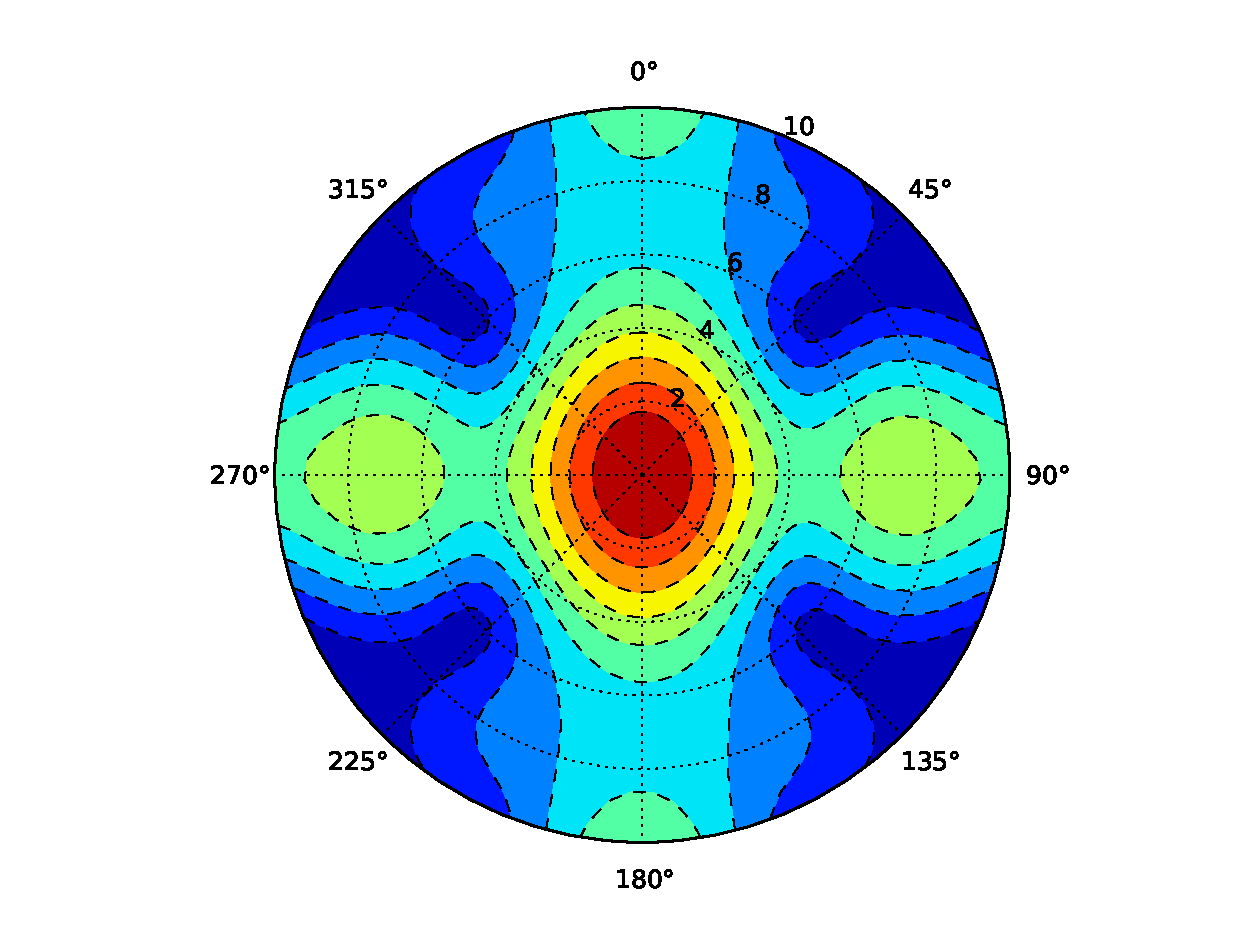
\includegraphics[width=8cm,height=6cm]{fig/chap2/arf_yka_1hz.eps}
}
\hfill{}\subfloat[\label{yka2}]{\centering %
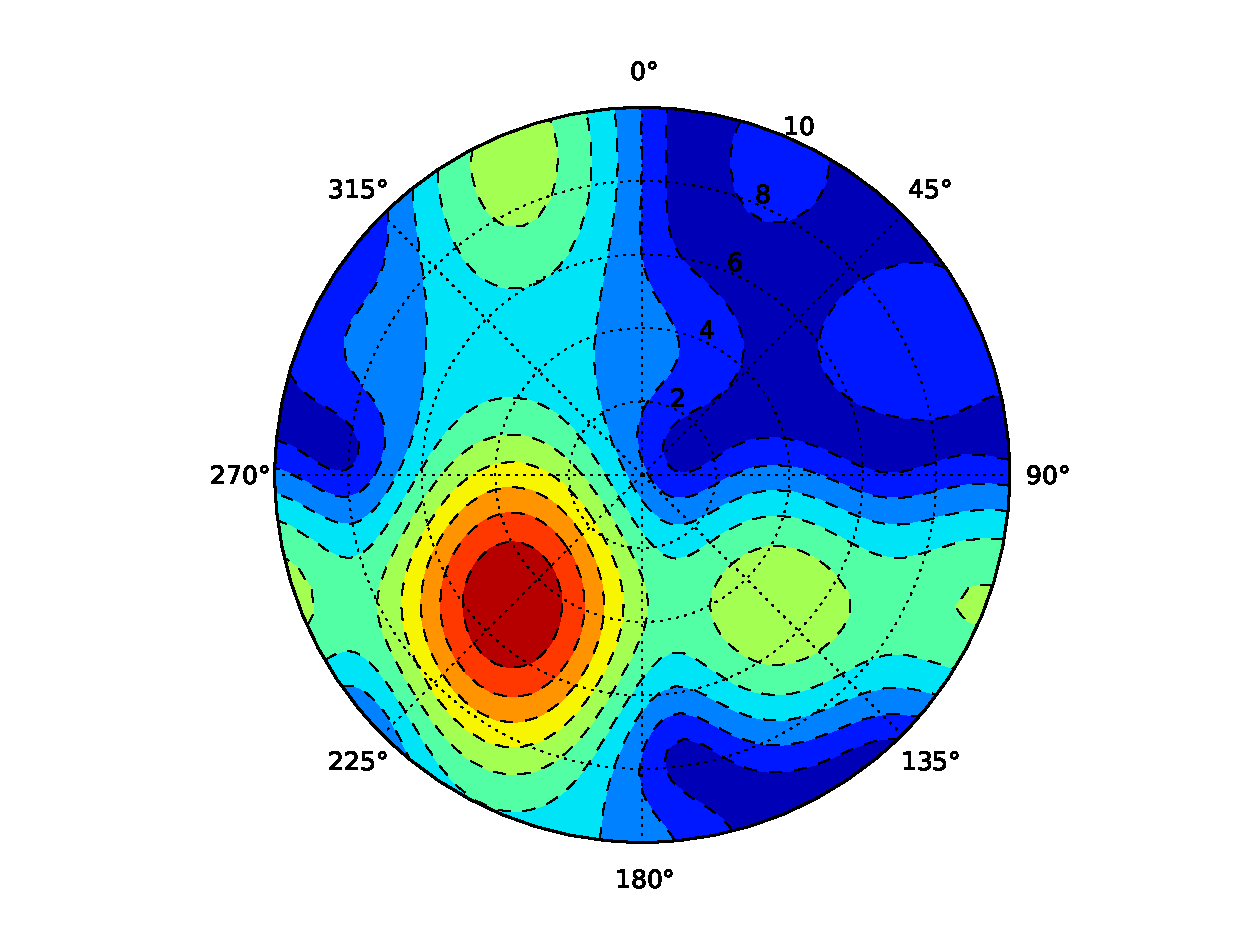
\includegraphics[width=8cm,height=6cm]{fig/chap2/arf_yka_1hz_2.eps}
}
\hfill{}
\caption{YKA台阵的ARF函数(a)$1HZ$的单色平面波从台阵正下方垂直入射的情况。%
(b)慢度$u=5 s/deg$的$1HZ$的单色平面波沿着反方位角$\theta = 225\textdegree$到达台阵的情况。}
\label{yka}
\end{figure}

\begin{figure}[tbph]
\hfill{}\subfloat[\label{grf1}]{\centering %
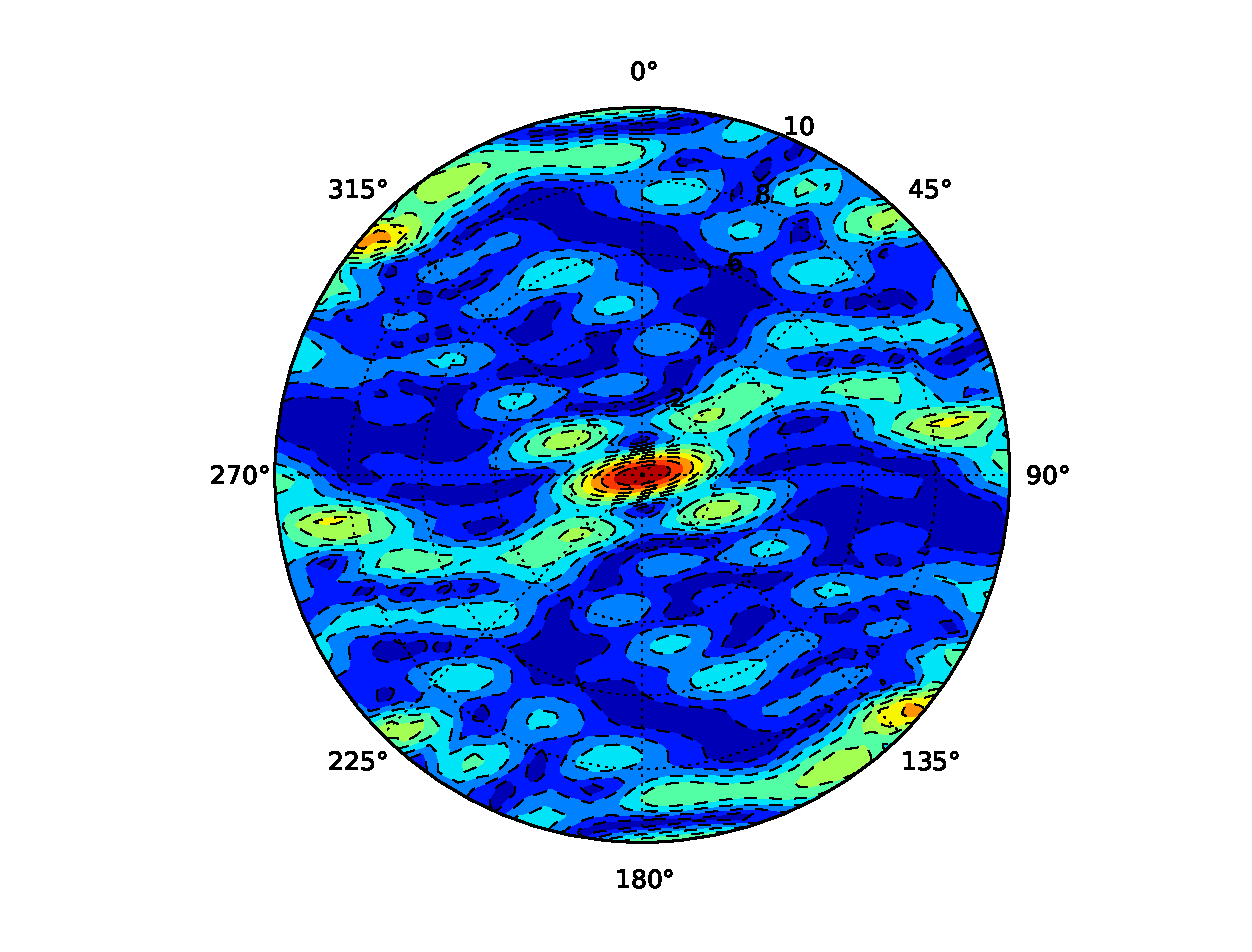
\includegraphics[width=8cm,height=6cm]{fig/chap2/arf_grf_1hz.eps}
}
\hfill{}\subfloat[\label{grf2}]{\centering %
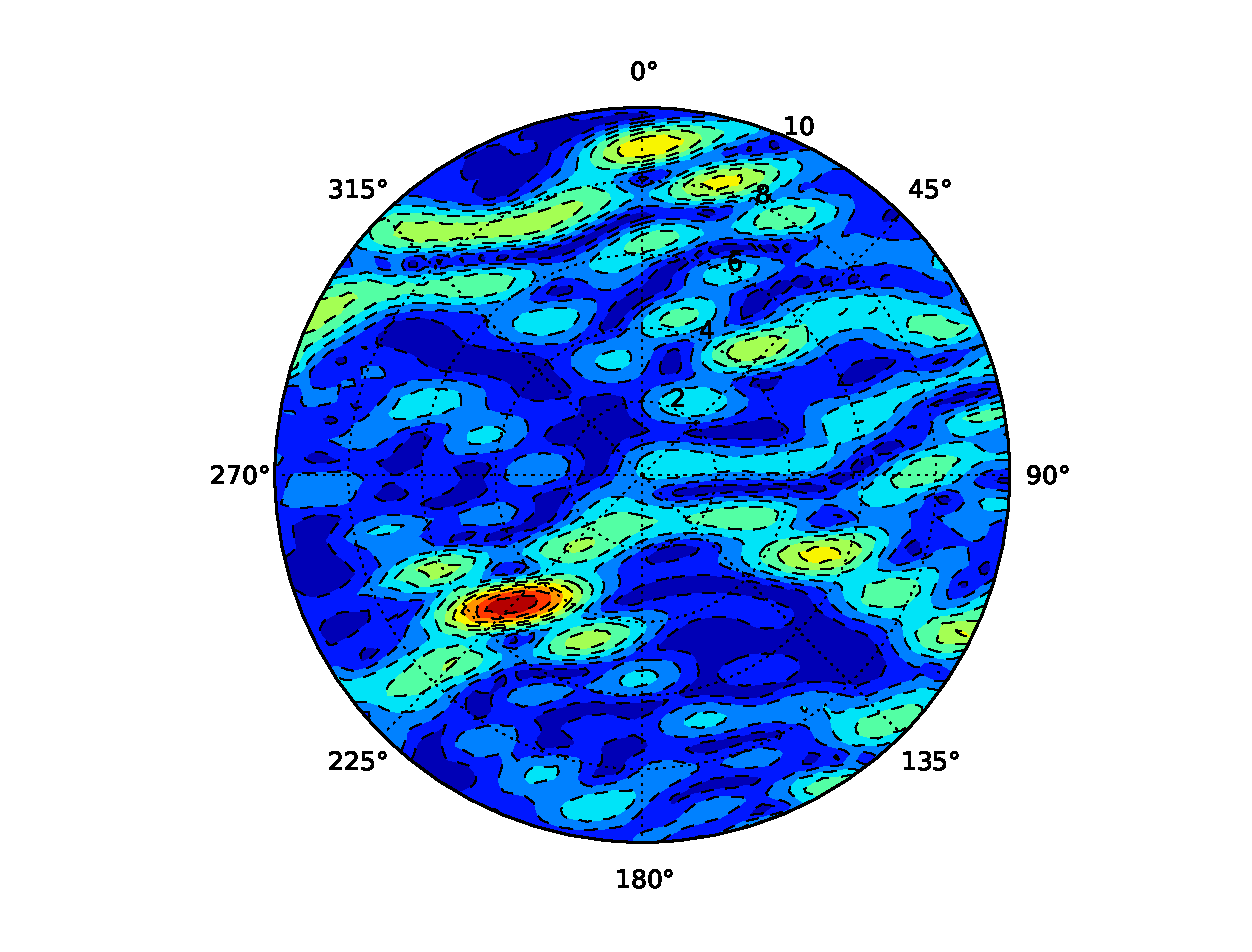
\includegraphics[width=8cm,height=6cm]{fig/chap2/arf_grf_1hz_2.eps}
}
\hfill{}
\caption{GRF台阵的ARF函数(a)$1HZ$的单色平面波从台阵正下方垂直入射的情况。%
(b)慢度$u=5 s/deg$的$1HZ$的单色平面波沿着反方位角$\theta = 225\textdegree$到达台阵的情况。}
\label{grf}
\end{figure}

图\ref{yka}和图\ref{grf}分别表示了YAK和GRF台阵的台阵响应函数(ARF),其中的(a)和(b)
分别对应信号从台阵正下方垂直到达台阵和以$u=5s/deg$的慢度从反方位角$225\textdegree$
到达台阵的情况。可以明显看出小口径的YKA台阵对慢度的分辨能力不佳,ARF函数有很大的主瓣。而
中型口径的GRF台阵慢度分辨率得到了明显提升,主瓣更小。同时由于GRF台阵并不规则,且口径较大,
因此其对来自不同反方位角的信号的分辨能力也不相同。其ARF函数的主瓣并不是呈圆形,而是长轴为
北偏东方向的椭圆,这使得其在北偏东方向上有较高的方位角分辨率,在这个方向上慢度大小分辨率
较低;反之在北西方向慢度分辨率较高,方位角分辨较低。

\subsection{不同频率下的ARF函数}

研究需要关注的不同震相信号其频率不相同,因此需要考察不同频率下台阵响应函数的形态,以此来评估台
阵对某特定频率信号的分辨能力。下面将以YKA、WRA和PSA几个小口径台阵为例子,比较它们在不同频率下的台阵响应函数,台阵的几何形状见图\ref{geometery}。


\begin{figure}[tbph]
\hfill{}
\subfloat[YKA]{%
\centering
\includegraphics[width=4cm,height=3.5cm]{fig/chap2/yka.eps}
}
\hfill{}
\subfloat[WRA]{%
\centering
\includegraphics[width=4cm,height=3.5cm]{fig/chap2/wra.eps}
}
\hfill{}
\subfloat[PSA]{%
\centering
\includegraphics[width=4cm,height=3.5cm]{fig/chap2/psa.eps}
}
\hfill{}
\caption{小台阵YKA、WRA和PSA的几何形状,其中的红色圆圈表示台站的位置。}
\label{geometery}
\end{figure}

三个小口径台阵的口径和台间距均类似,分别为2公里和20公里,只是形态不同。YKA台阵是由两条线状
台阵交叉而成;WRA台阵由从一点出发的两条线状台阵组成,开口向东北方向;PSA台阵则呈现规则的
螺旋形状。图\ref{freq}显示了分别在频率为$1Hz$和$2Hz$情况下,三个台阵的ARF函数。

\begin{figure}[tbph]
\hfill{}
\subfloat[]{%
\centering
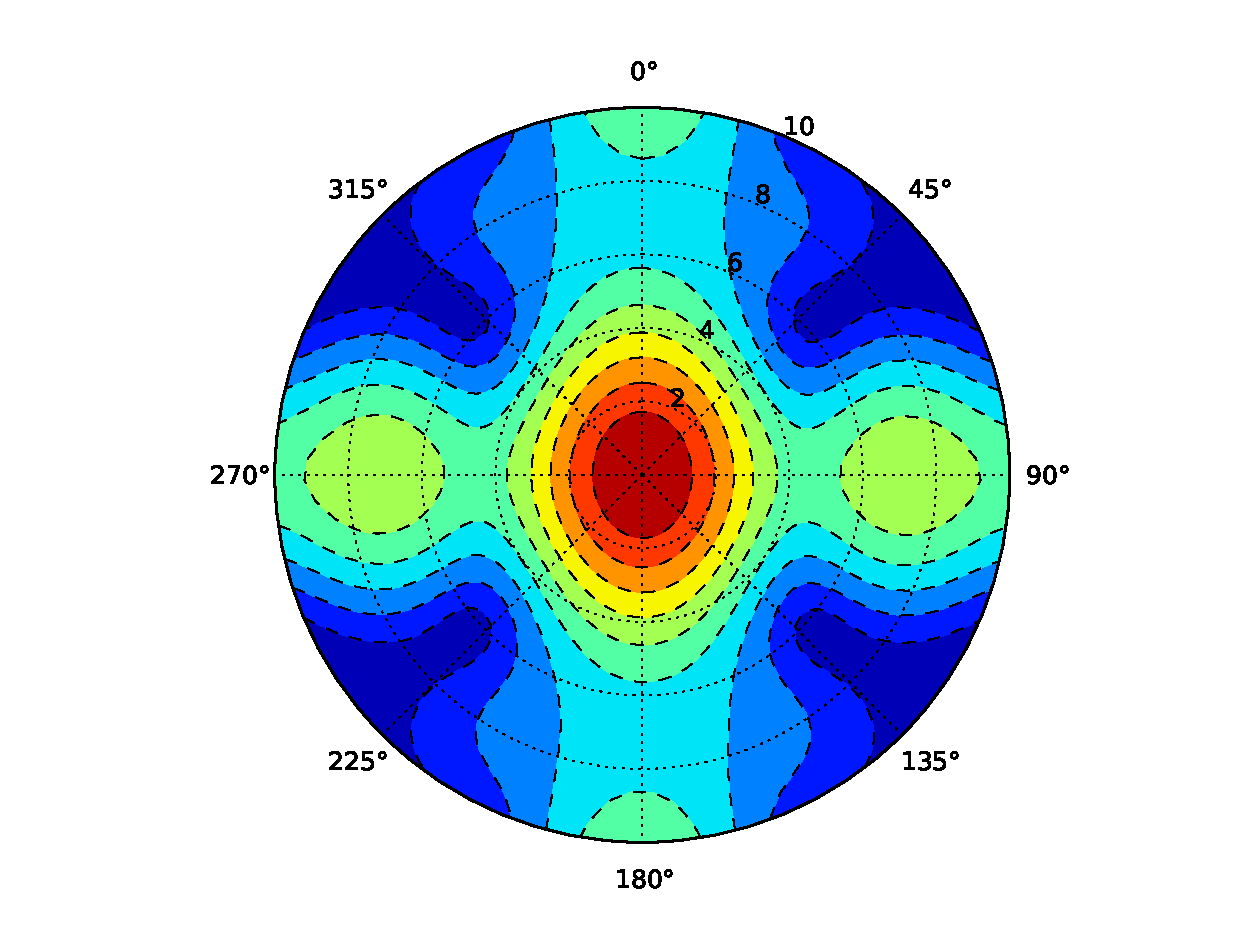
\includegraphics[width=8cm,height=6cm]{fig/chap2/arf_yka_1hz.eps}
}
\hfill{}
\subfloat[]{%
\centering
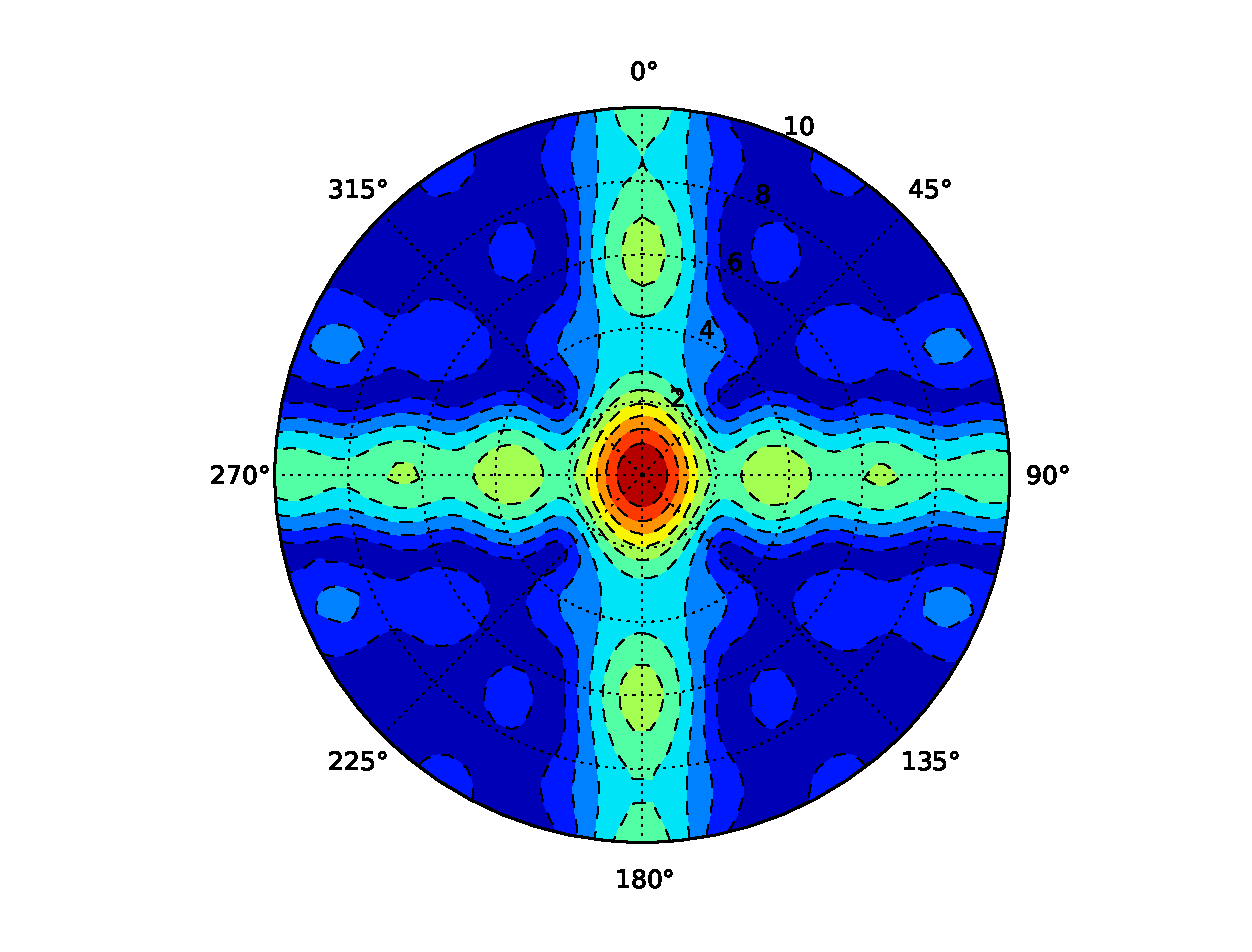
\includegraphics[width=8cm,height=6cm]{fig/chap2/arf_yka_2hz.eps}
}
\hfill{}\\
\hfill{}
\subfloat[]{%
\centering
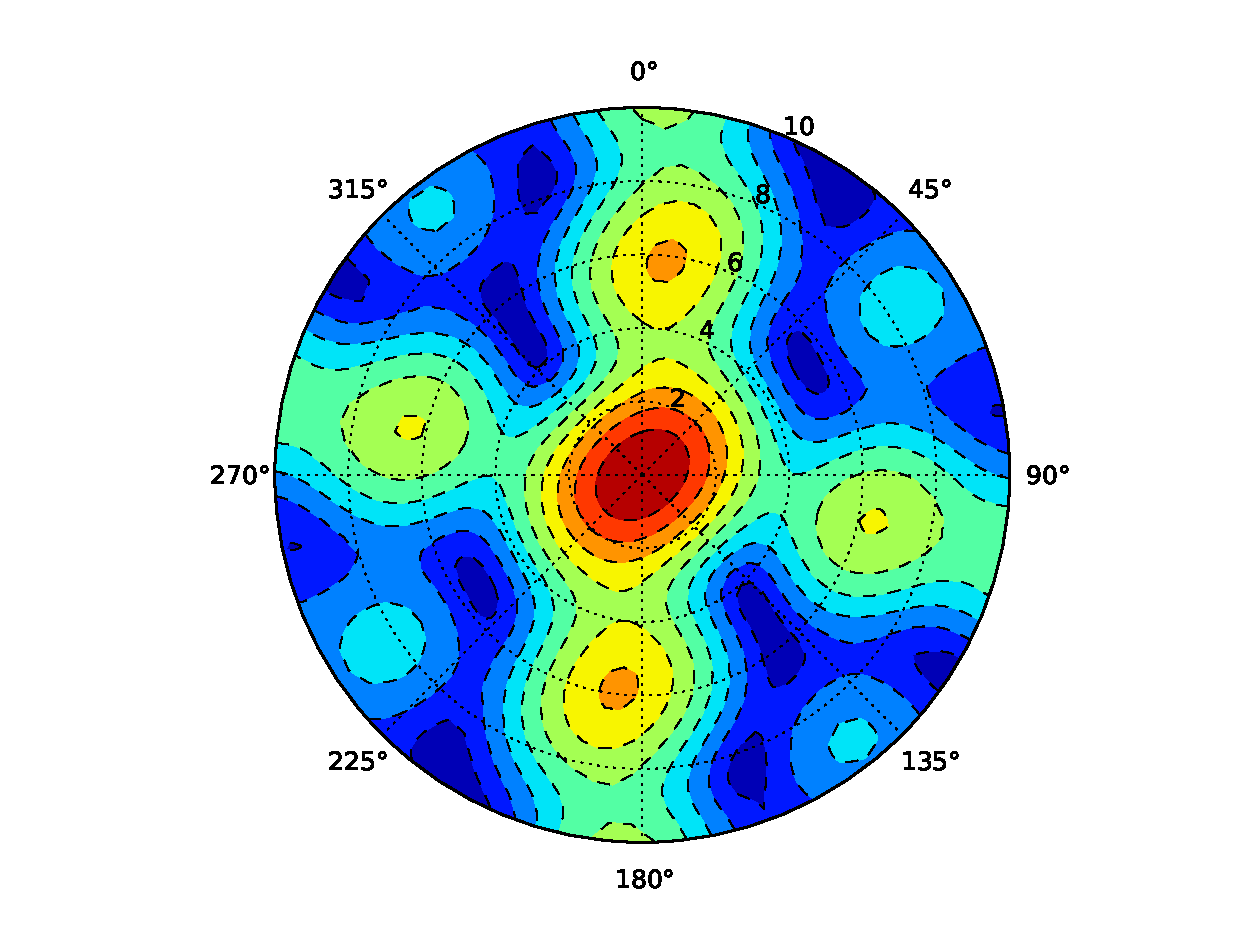
\includegraphics[width=8cm,height=6cm]{fig/chap2/arf_wra_1hz.eps}
}
\hfill{}
\subfloat[]{%
\centering
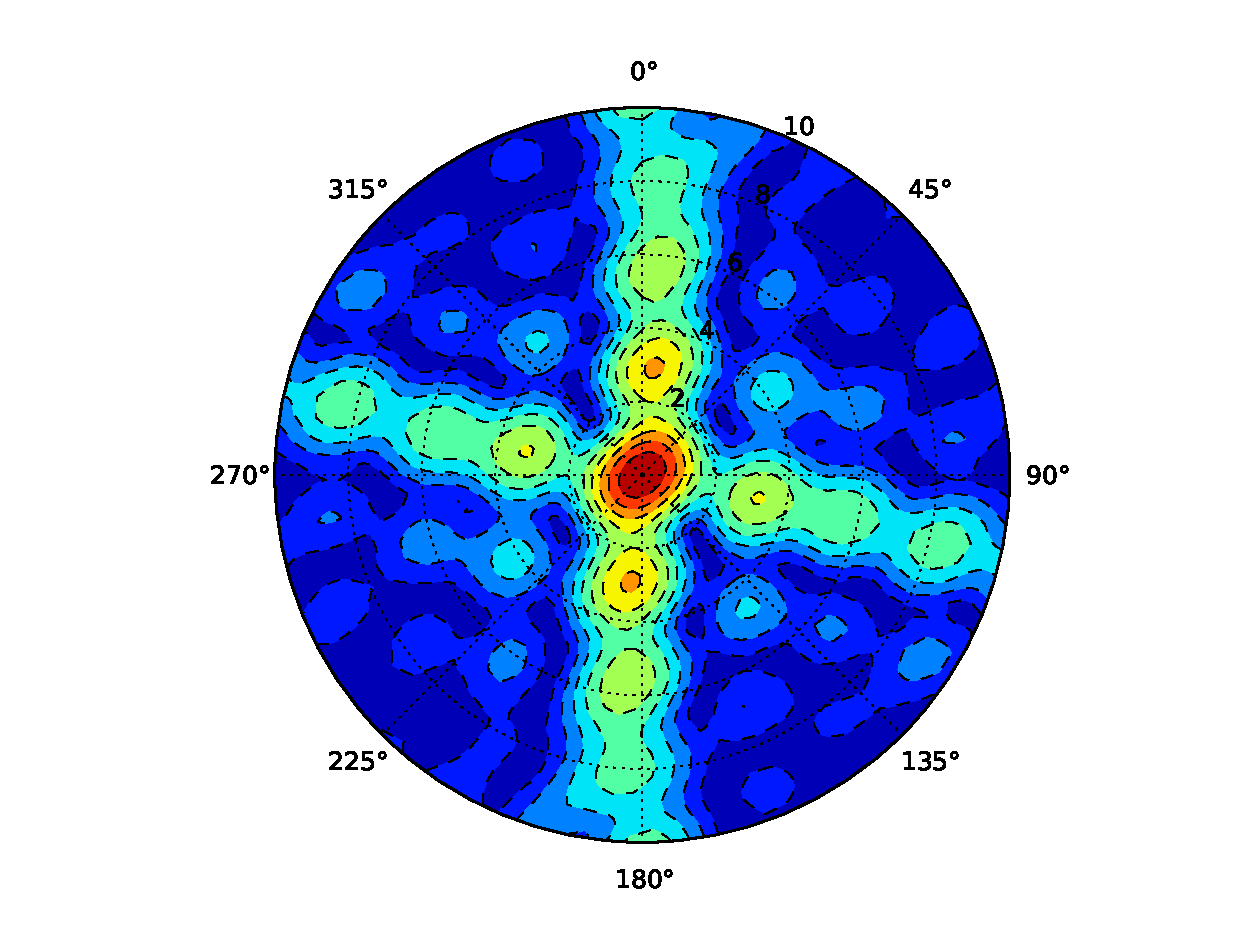
\includegraphics[width=8cm,height=6cm]{fig/chap2/arf_wra_2hz.eps}
}
\hfill{}\\
\hfill{}
\subfloat[]{%
\centering
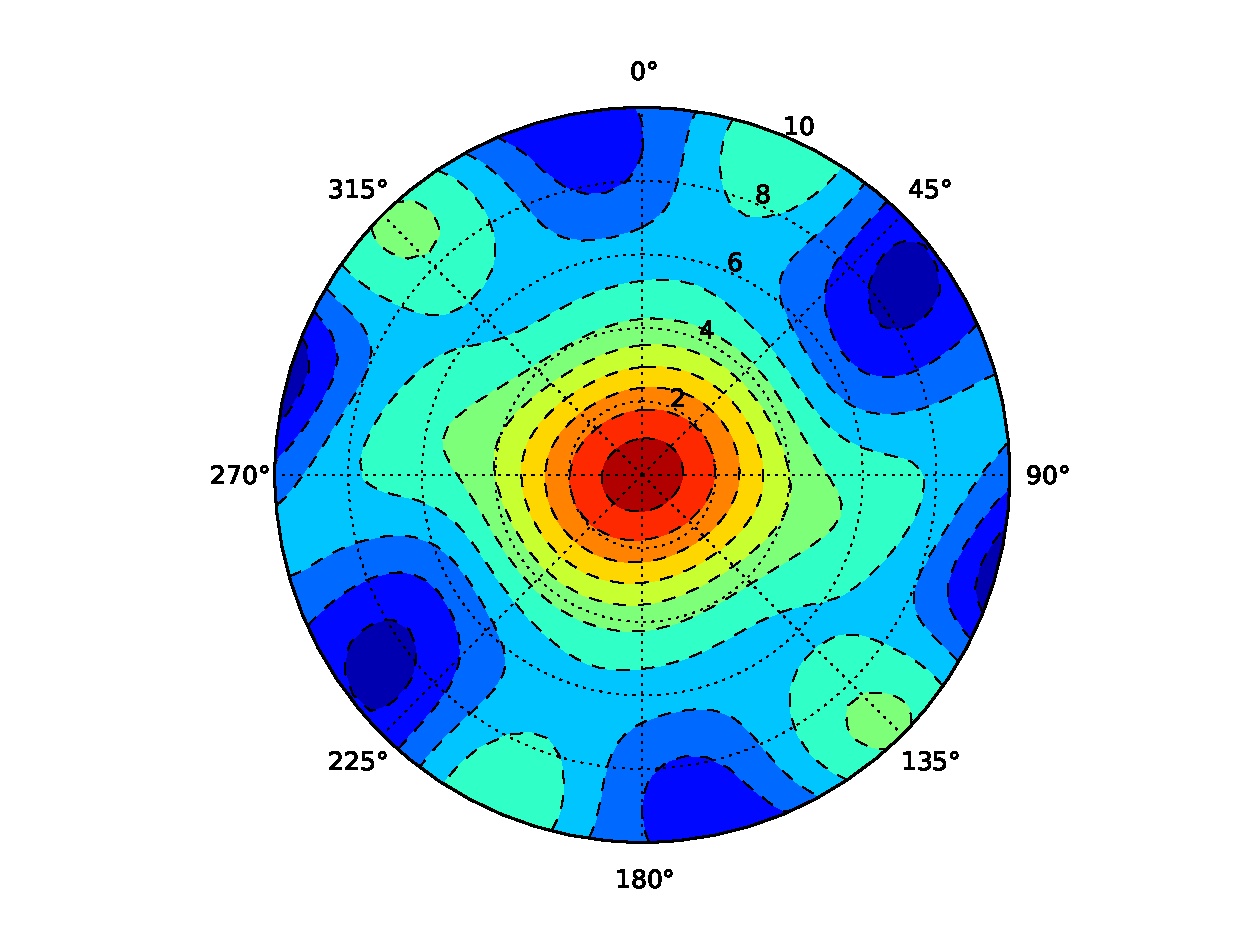
\includegraphics[width=8cm,height=6cm]{fig/chap2/arf_psa_1hz.eps}
}
\hfill{}
\subfloat[]{%
\centering
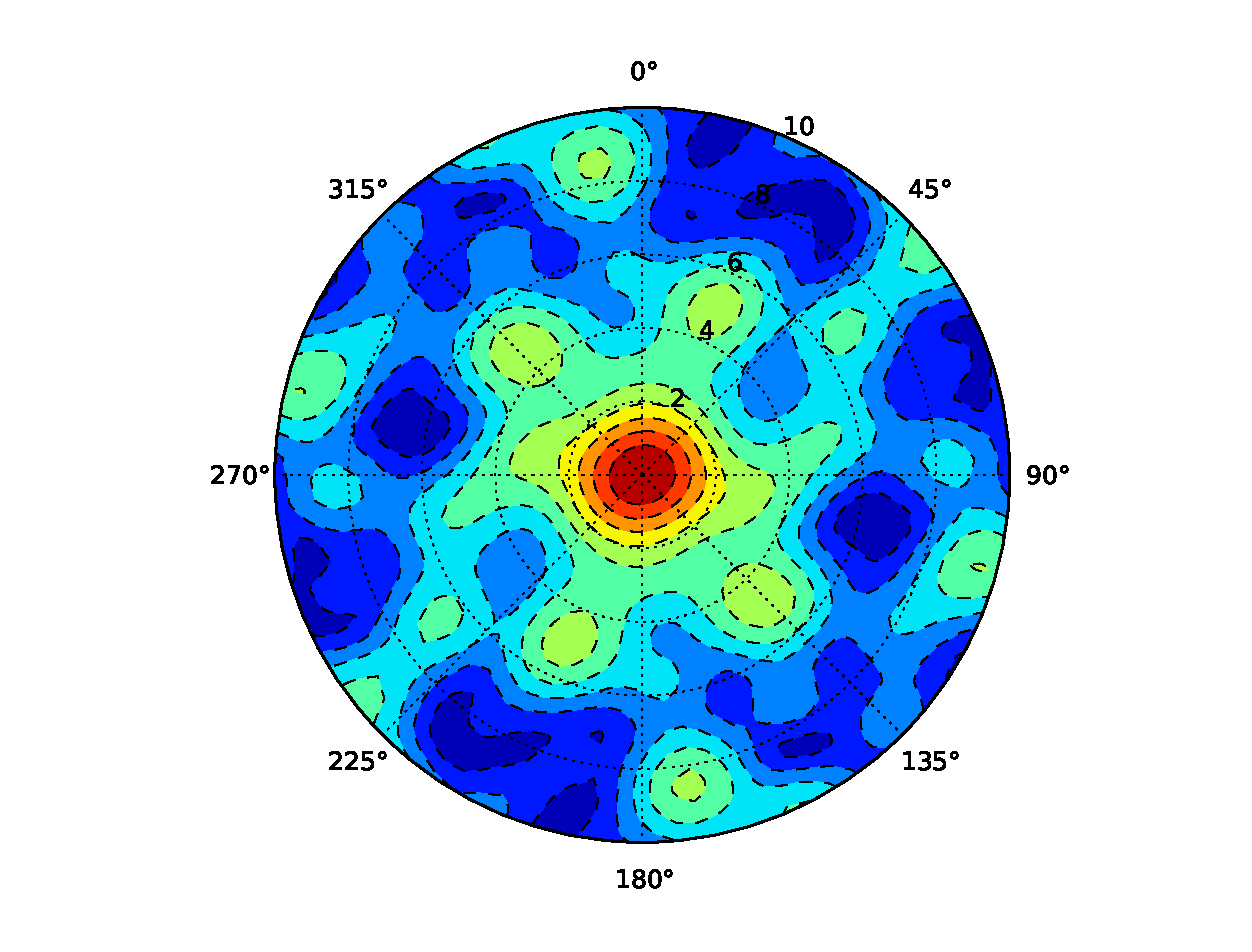
\includegraphics[width=8cm,height=6cm]{fig/chap2/arf_psa_2hz.eps}
}
\hfill{}
\caption{(a)、(b)YKA台阵在1Hz和2Hz下的ARF函数;(c)、(d)WRA台阵在1Hz和2Hz下的ARF函数;%
(e)、(f)PSA台阵在1Hz和2Hz下的ARF函数}
\label{freq}
\end{figure}

图\ref{freq}显示,随着所接收的信号频率增大,台阵乡响应函数的主瓣缩小,变得更加尖锐,对慢度的
分辨力提高,频率$\omega$只起到一个缩放因子的作用;但由于口径均较小,三个台阵对慢度的分辨
能力差异不是很大,ARF函数主要受到口径和台间距影响,台阵几何形状的对ARF函数形态贡献较小。


\section{相位加权叠加(Phased-Weighted Stack)}

PWS方法最早见于地幔间断面转换波的探测\citep{Schimmel1997},能够增强连续的一致信号,压制不连续的随机噪声,目前较为广泛地用于弱信号的识别。典型的例子就有用与前临界PKiKP的研究
\citep{Koper2003,Koper2004},还有用于寻找穿过内核的S波震相PKJKP\citep{Deuss2000}。下面将简要介绍PWS方法的原理还有与Slant叠加的效果对比。

\subsection{PWS方法原理}

PWS是一种非线性叠加方法,它使用一种不依赖振幅的一致性度量方法来加权线性叠加。在叠加的过程中
首先要构建一个解析复信号$S(t)$,它的实部是台站接收到的信号$s(t)$,虚部是则是实部的希尔伯特
变换

\begin{equation}
S(t) = s(t) + i \mathscr{H} [s(t)]
\end{equation}

上式可以写成振幅和相位分离的形式

\begin{equation}
S(t) = A(t) exp[i \Phi (t)]
\end{equation}

其中$A(t)$是地震信号的波包,$\Phi (t)$为瞬时相位。相位叠加的表达式如下

\begin{equation}
c(t) = \frac{1}{N} \left| \sum_{j=1}^{N} exp[i \Phi_j (t)] \right|
\end{equation}

用相位的$\nu$次幂作为加权系数,就得到了PWS的表达式

\begin{equation}
 \nu_{PWS}(t) = \frac{1}{N} \sum_{j=1}^{N} s_j (t)c^{\nu} (t)
\end{equation}

\subsection{PWS与倾斜叠加观测对比}

与简单的线性叠加相比,PWS压制噪声的优势非常明显,能有效突出弱型号。图\ref{compare}
比较了Hi-net~27个台站在PKiKP理论时窗附近的叠加结果,事件位于19.35N,144.76E,震源
深度446.9公里,时间是2010年3月8日。27个台阵位于19.78$\textdegree$至
20.78$\textdegree$的震中距范围内,理论慢度为0.449s/deg,理论到时为942.62s。

\begin{figure}[tbph]
\centering
\subfloat[]{ %
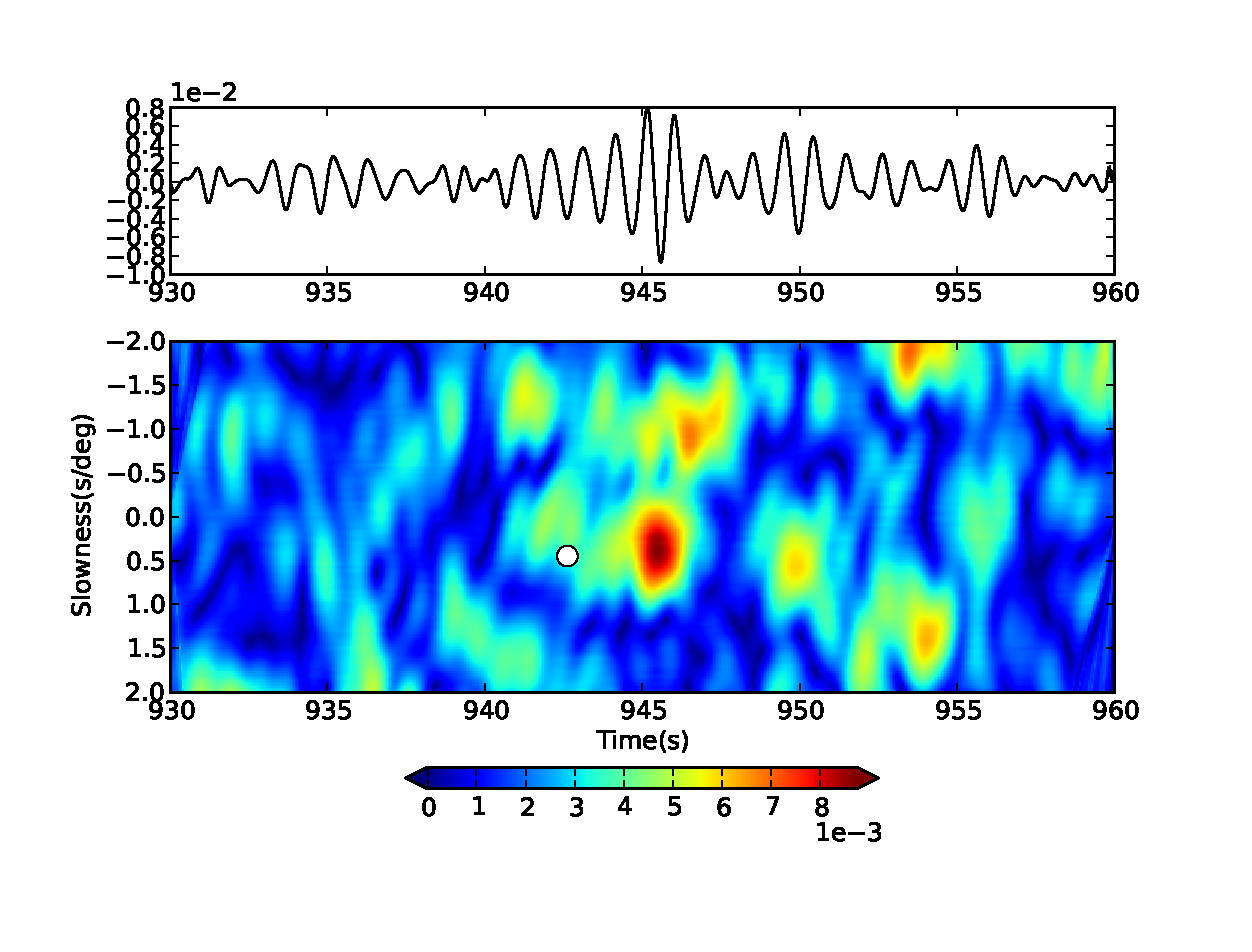
\includegraphics[width=14cm,height=10cm]{fig/chap2/slant_2846275.eps}
}\\
\subfloat[]{ %
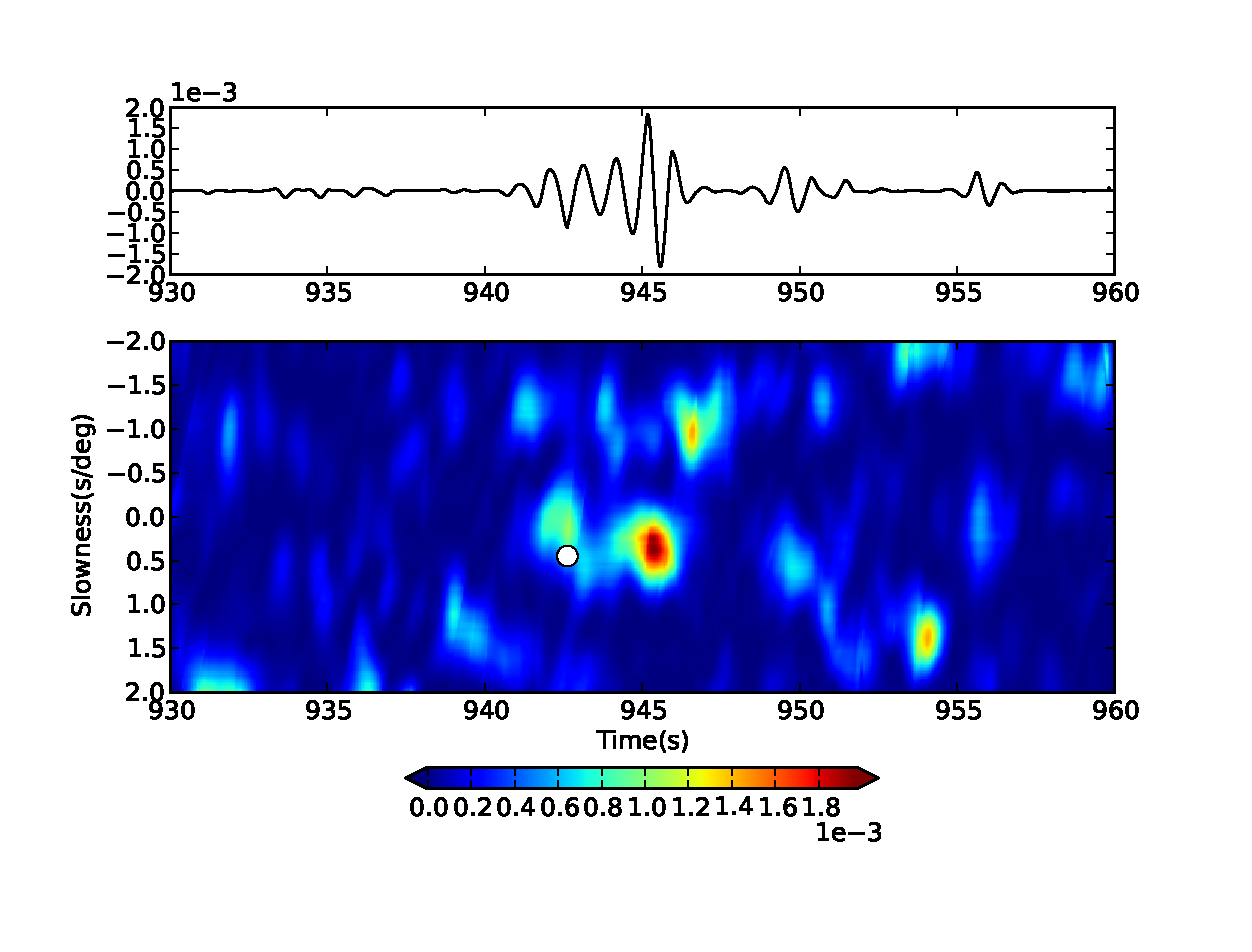
\includegraphics[width=14cm,height=10cm]{fig/chap2/pws_2846275.eps}
}\\
\caption{Slant叠加与PWS的结果对比(a)Slant叠加的结果(b)PWS的结果。上面的部分是叠加最%
大能量出的波形。叠加的慢度搜索间隔是0.02s/deg,白色圆圈表示理论慢度和到时的位置,%
u=0.449s/deg,t=942.62s}
\label{compare}
\end{figure}

可以看出,虽然两种叠加方法得到的最大能量与理论慢度都很接近,但是线性叠加的结果,波包最大能
量处附近还有其他较大的能量区域分布,而PWS则将这些噪声压制得比较干净,从叠加最大能量处的波形看
,PWS的效果也明显更好。图是叠加用到的27道数据,单从波形看,很难分辨出有效信号,在理论到时前后
均有比较大的振幅。

\begin{figure}[tbph]
\centering
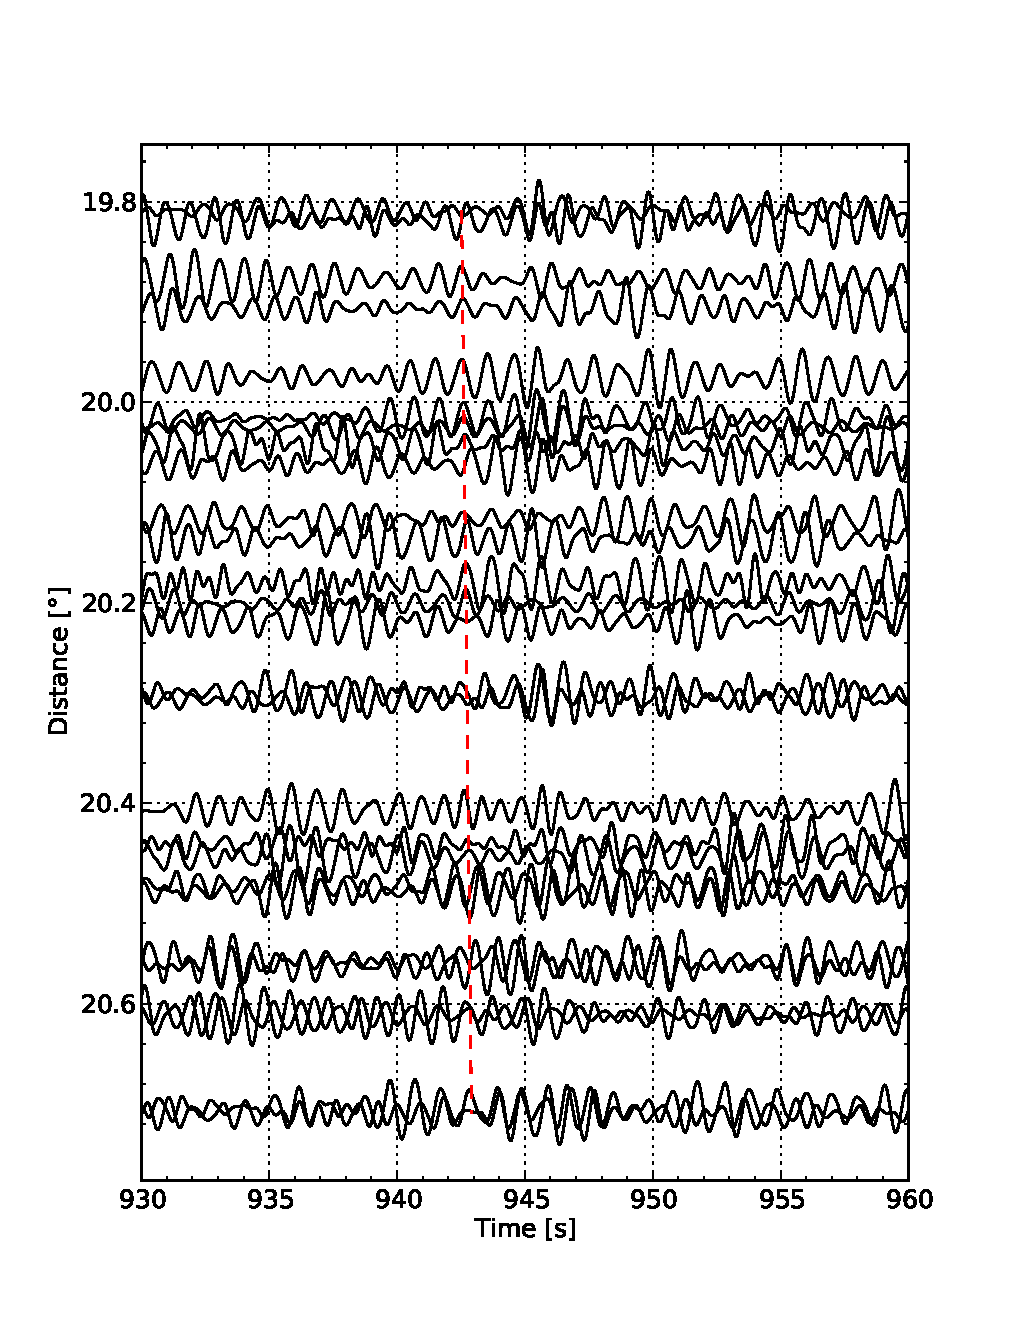
\includegraphics[width=12cm,height=16cm]{fig/chap2/section.eps}
\caption{27道Hi-net台站波形数据,按震中距从小到大排列,其中红色的虚线表示的是PKiKP的理论到时。}
\label{section}
\end{figure}

\begin{figure}
\centering
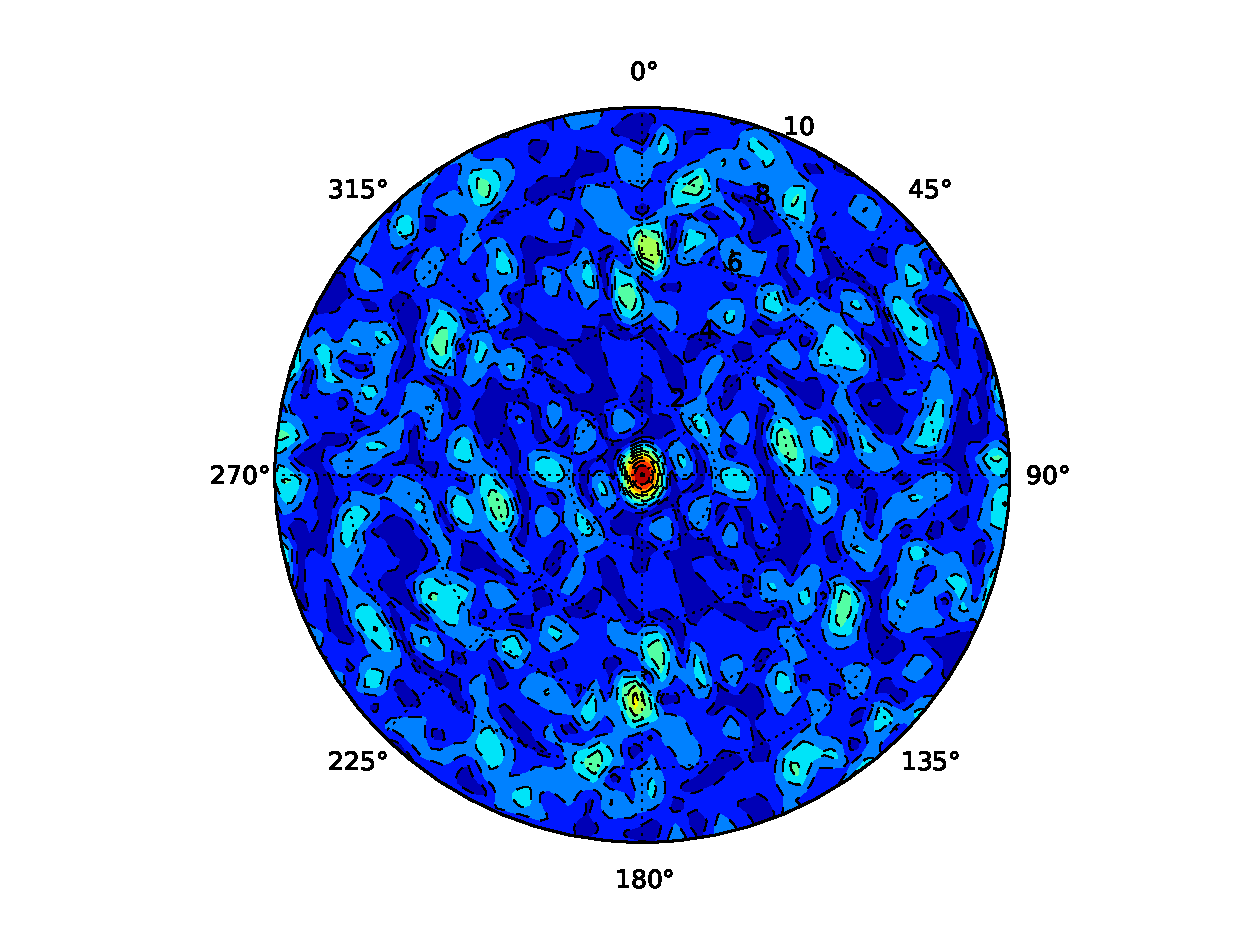
\includegraphics[width=10cm,height=8cm]{fig/chap2/arf_hinet.eps}
\caption{27个台站组成的台阵的ARF函数}
\end{figure}

%\chapter{Data and Observation}


\section{Observation of Global subcritical PKiKP}

自地球内核被发现以来~\citep{lehmann1936p}已经过去将近70年,正是由于在之前被认为是内核影区的
地方发现了来自内核的绕射震相,即后临界PKiKP,才证实了内核的存在。但是由于内外核界面反射系数较小,
相比与其他界面的反射震相如PcP,前临界PKiKP的振幅很微弱,一般为PcP振幅的数十分之一,PKIKP的十分
之一左右~\citep{Bolt1965},要观测到它需要很高的信噪比,这对仪器和环境的要求也就随之提高。在内核的存在被证实后的几十年,作为其存在更为直接证据的前临界PKiKP的观测都没有报道。上世纪70年代,随着
地震台阵的发展,有关前临界PKiKP的观测结果才开始出现~\citep{Engdahl1970a}。但在单道上观测前
临界PKiKP非常困难,\citep{Shearer1990}在数万道记录中也只找到两个疑似的PKiKP相位,即使在PKiKP理论到时附近存在一个大于噪声级别的振幅,也难以断定其就是PKiKP相位。

\begin{figure}[!ht]
	\hfill{}
	\subfloat[]{\centering%
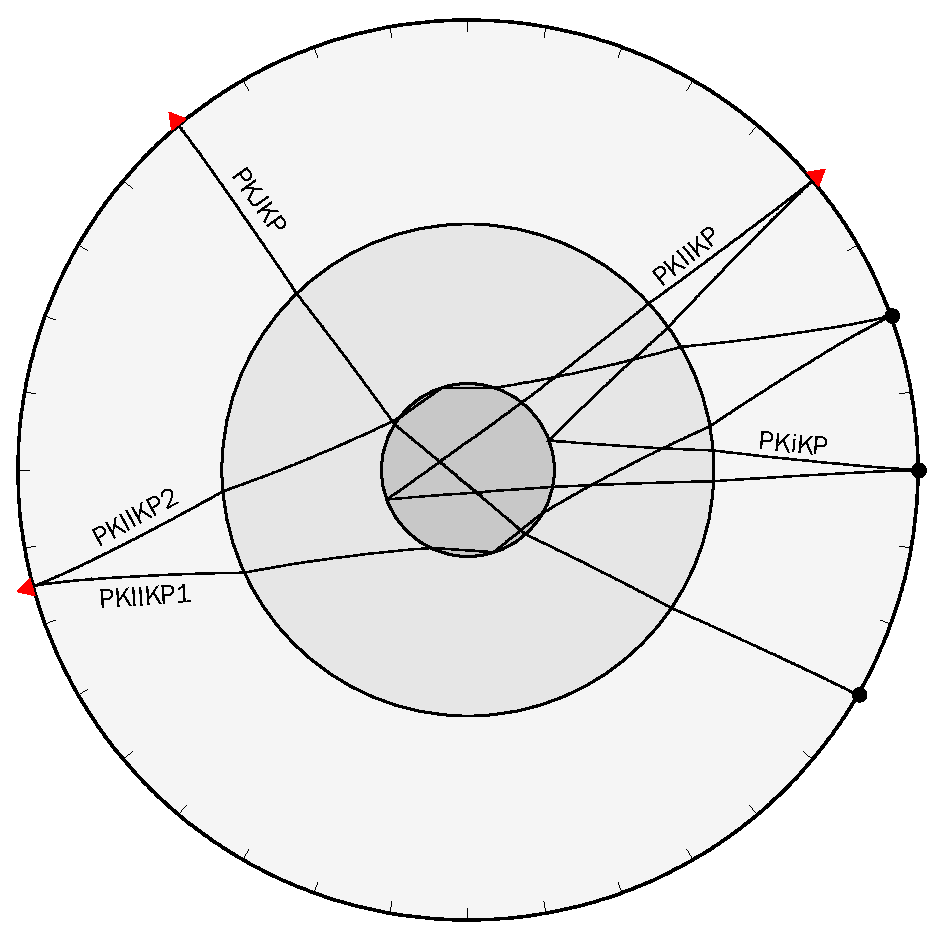
\includegraphics[width=6cm,height=6cm]{fig/chap3/path.eps}
}
	\hfill{}
	\subfloat[]{\centering%
\includegraphics[width=6cm,height=6cm]{fig/chap3/time.eps}
}
	\hfill{}
	\caption{Seismic phases which samples inner core, and their travel time %
curve.}
\end{figure}

要得到确定性的前临界PKiKP观测必须要用到台阵,而目前用来寻找前临界PKiKP的台阵又分为两种,其一是微型台阵,口径从几公里到十几公里,例如IMS台阵;其二是区域密集型台阵,口径数百公里,台站数量在几百个左右,典型的有Hi-net、USArray和阿拉斯加区域台网等。微型台阵虽然台站数量少往往在十个左右,但是能
够用于快速寻找微弱震相。因为就台阵口径而言,传播到台阵上的波已经可以看作平面波,即可以认为每个台站
接收到的是同一信号,如果在每个台站上都能看到这个相位,这就排除了特定区域的随机噪声的因素。而且当
台站间距足够小的时候,直接将所有信号直接相加就足以起到提高信噪比的作用;大口径密集台阵的优势在于, 台阵的数量还有其震中距的跨度,即增大了发现某一地震产生的前临界PKiKP相位的概率,如果台站足够多,
则能得到足够数量的PKiKP观测,再通过慢度分析就可以确定信号的来源。

最早使用微型台阵寻找前临界PKiKP的是~\cite{Souriau1989},利用WRA台阵并运用叠加方法观测到了PKiKP,由于年代较早,受限与仪器等因素,并没有在单道上看到清晰的、高信噪比的PKiKP相位。在十多年后,
\cite{Koper2003}利用全球的IMS微型台阵从1995至2000年间的数据,用台阵方法找到了数百对的PKiKP和PcP波形;而\cite{Kawakatsu2006}则利用Hi-net近700个台站的数据,观测到了自同一事件的清晰的前临界PKiKP,通过慢度分析和波形拟合,有力地证实了存在尖锐的ICB。值得注意的是,虽然相比于较早的研究
,更多的前临界PKiKP已经被发现和确认,但数据覆盖依然有限,可以看出,\cite{Koper2003}的研究中
PKiKP在ICB反射点的分布主要集中在环太平洋区域,欧亚大陆下方的ICB则没有覆盖,而且PKiKP虽然数量增
多,但很多来源与相邻的地震,其在ICB的采样点的并不具有均匀的分布,因此之前的研究未能给出ICB全球
范围的特征,区域的ICB特征也不能给出清晰的全球范围的动力学指示。

\subsection{Data}

本文除了用到先前研究所用到的IMS台阵的数据,还增加了中亚哈萨克斯坦、苏格兰、中欧还有北欧的IMS小台阵数据,而且澳大利亚及美国的IMS台阵也有所增加,所有IMS台阵的数据均从Iris数据中心获得,但先前研究
用到的CMAR和KSAR等台阵的数据不能获取。
所用到的台阵数据如下:澳大利亚的ASAR(2012-2013)、WRA(2010-2012)、PSAR(2012-2015);北美的BCAR、BMAR和IMAR(2013.11-2015.5),YKA(2013.7-2014.11),NVAR(1998-2014),ILAR,TXAR,PDAR;哈萨克斯坦的ABKAR,KKAR,MKAR;德国的GERES;
罗马尼亚的BURAR;苏格兰的EKB;挪威的SPB。所有的地震事件均选取5级以上,震中距从10到70度,震源
深度没有限制。所有的IMS台站数据均通过1-2Hz的滤波,所有的事件均通过手工挑选,保证数据的质量。
观测到的PKiKP的事件与台阵分布如图\ref{distibution},其中包含了每道都具有清晰的PKiKP相位的观测和需要叠加才能看到清晰PKiKP相位的观测。可以看到PKiKP的IMS台阵的震中距主要集中在20~40度之间,这也是前临界PKiKP在ICB反射系数最大的区间。

除了小口径台阵,这里还增加了部分阿拉斯加区域台网AK、USarray以及Hi-net的数据,观测到PKiKP相位
的震中距范围在10至50度之内。在之前的研究中除了在Hi-net上,很少有在其他台网上观测到PKiKP的报道,
追究其原因可能是,对于密集台站的台网,从大量的事件中寻找到某个能产生可观测到的PKiKP信号很困难,
这需要进行大量的数据挑选。如果台站数量达到数百个,几千个事件就会有数十万道数据的挑选工作量,但其中
可能仅有数十个事件产生的PKiKP震相能被清晰地观测到。由于PKiKP的振幅受到的影响包括(1)震源辐射花样;(2)PKiKP射线在ICB反射点的性质;(3)震源到台站路径所经过的结构效应,观测到清晰PKiKP相位需要
合适的条件。因此这里提供一种能快速找到大量PKiKP相位的方法,即先用IMS小口径台阵搜索出能产生清晰
观测的事件,这些事件就是符合产生可观测到的前临界PKiKP震相条件的,然后用附近的密集台阵数据针对某一事件搜寻PKiKP震相,这样能显著提高搜索的效率。这里就用这种方法,在AK和USArray上找到了数十道清晰的
PKiKP相位,震中距的跨度甚至能超过20度,这些是之前的研究从未观测到的结果,关于它们的情况,后面会再次提到。

\begin{figure}
	\centering
	\subfloat[]{%
\includegraphics[width=12cm,height=6cm]{fig/chap3/global.eps}
}
\\
	\subfloat[]{%
\includegraphics[width=9cm,height=6cm]{fig/chap3/hist_dist.eps}	
}
	\caption{(a)观测到PKiKP的IMS小口径台阵和事件的全球分布。红色五角星表示地震,黑色三角形%
表示台阵,黑线表示射线路径的投影。(b)所有观测到PKiKP的IMS台阵数随震中距的分布直方图。}
	\label{distibution}
\end{figure}

\subsection{Observation from global IMS stations}

下面给出全球IMS台阵观测到的清晰PKiKP记录的例子,作为对照,同时附上PcP的记录。

\subsubsection{YKA}

\begin{figure}[!ht]
	\centering
	\subfloat[]{%
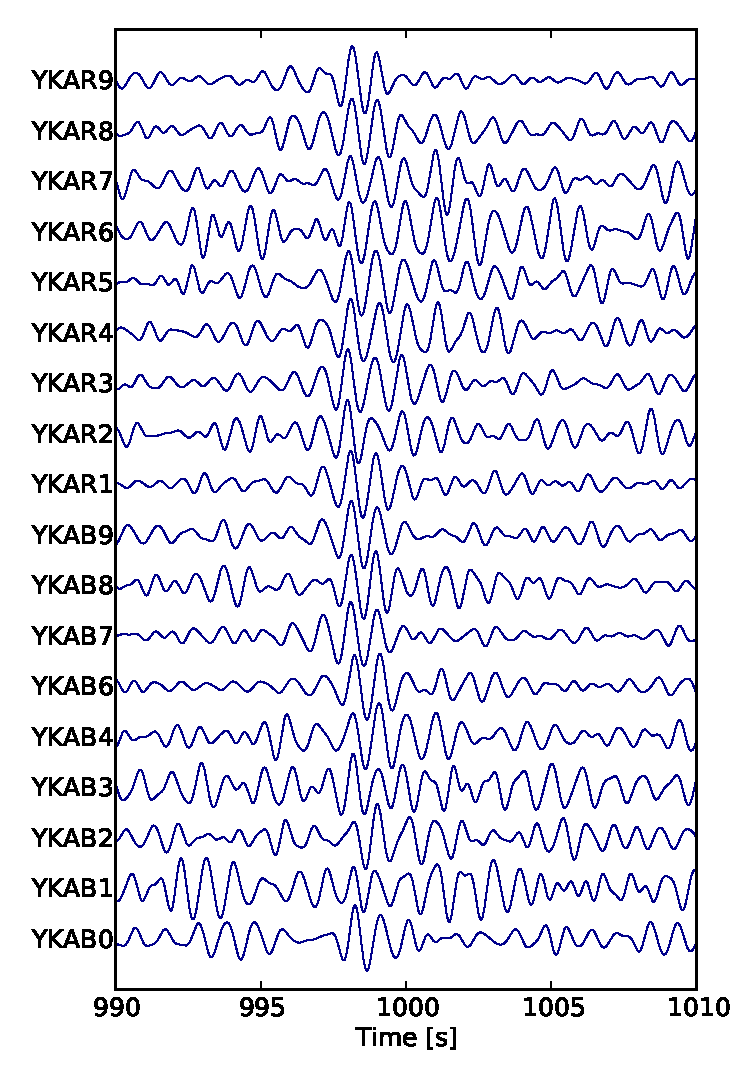
\includegraphics[width=5cm,height=8cm]{fig/chap3/4599655_pkikp_sec.eps}
}
	\hspace{2em}
	\subfloat[]{%
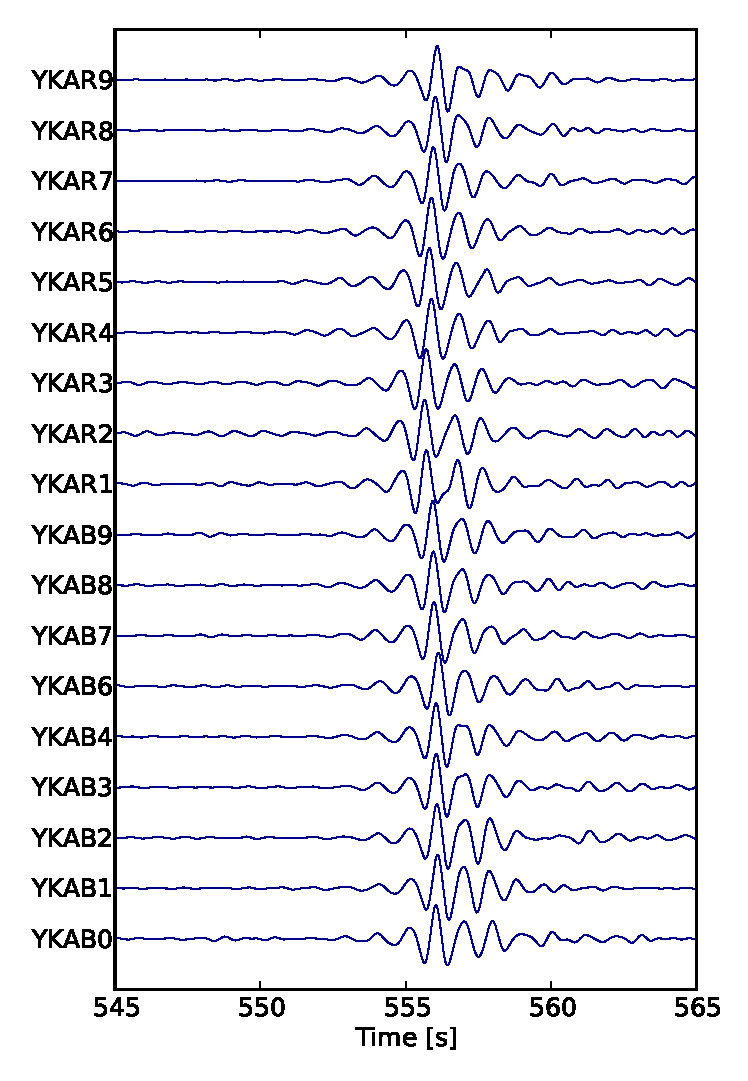
\includegraphics[width=5cm,height=8cm]{fig/chap3/4599655_pcp_sec.eps}
}
	\\
	\subfloat[]{%
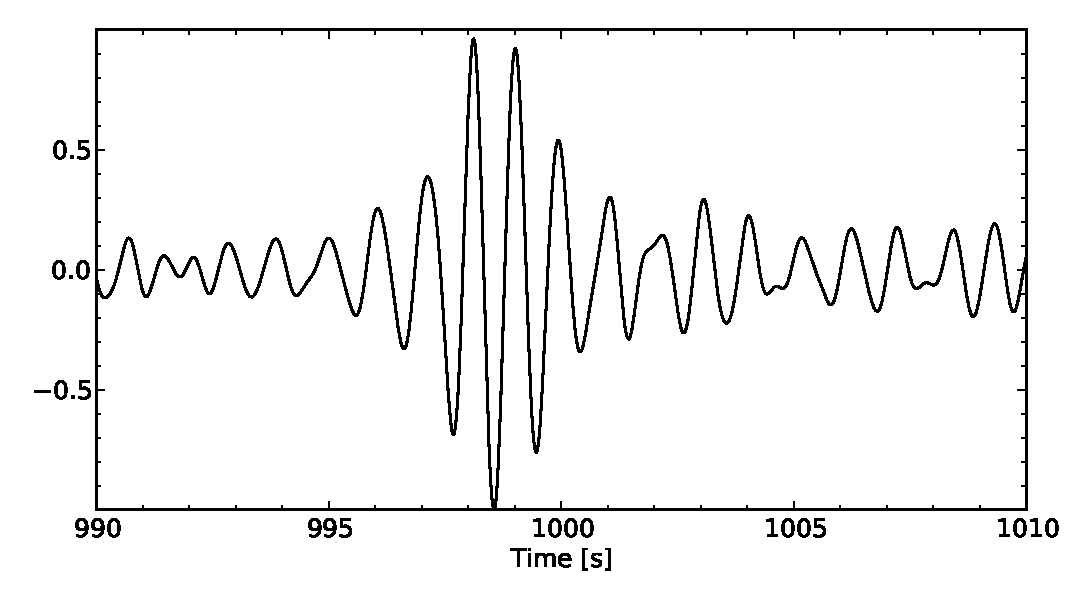
\includegraphics[width=5cm,height=2.5cm]{fig/chap3/4599655_pkikp_stack.eps}
}
	\hspace{3em}
	\subfloat[]{%
\includegraphics[width=5cm,height=3cm]{fig/chap3/4599655_yka_loc.eps}
}
	\caption{(a)YKA台阵的PKiKP记录(b)PcP所有单道记录(c)线性叠加后的PKiKP波形(d)事件和%
YKA台阵的位置关系,和地震的震源机制。}
\end{figure}

\newpage

\subsubsection{NVAR}

\begin{figure}[!ht]
	\centering
	\subfloat[]{%
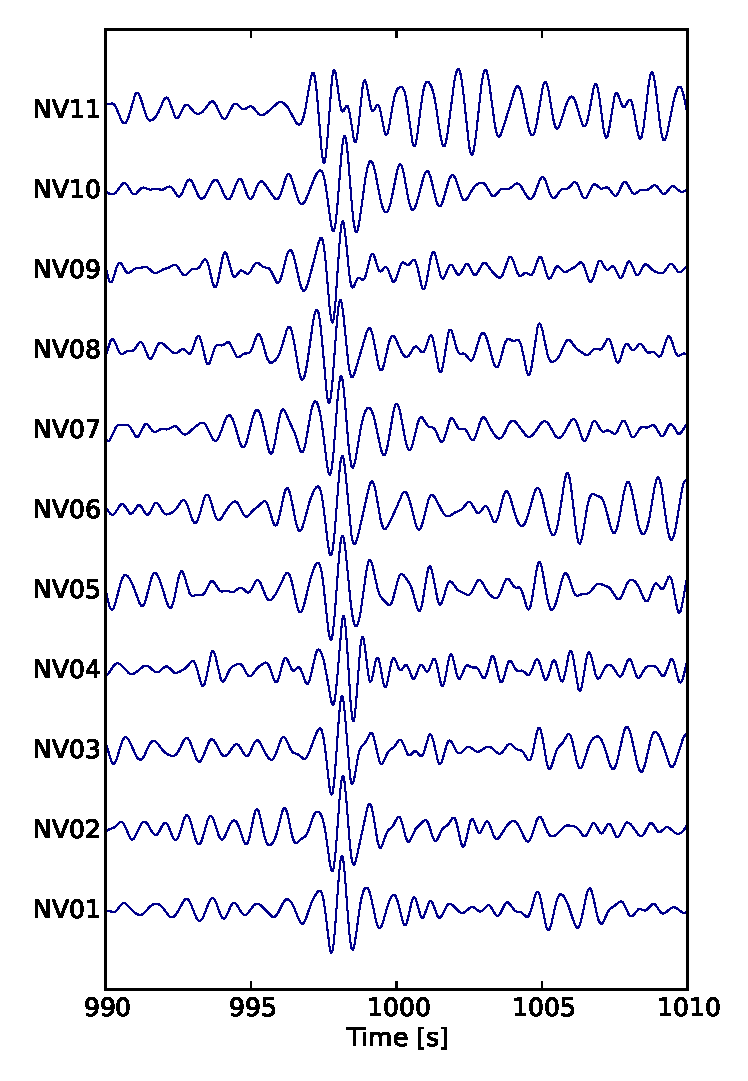
\includegraphics[width=5cm,height=8cm]{fig/chap3/4371355_pkikp_sec.eps}
}
	\hspace{2em}
	\subfloat[]{%
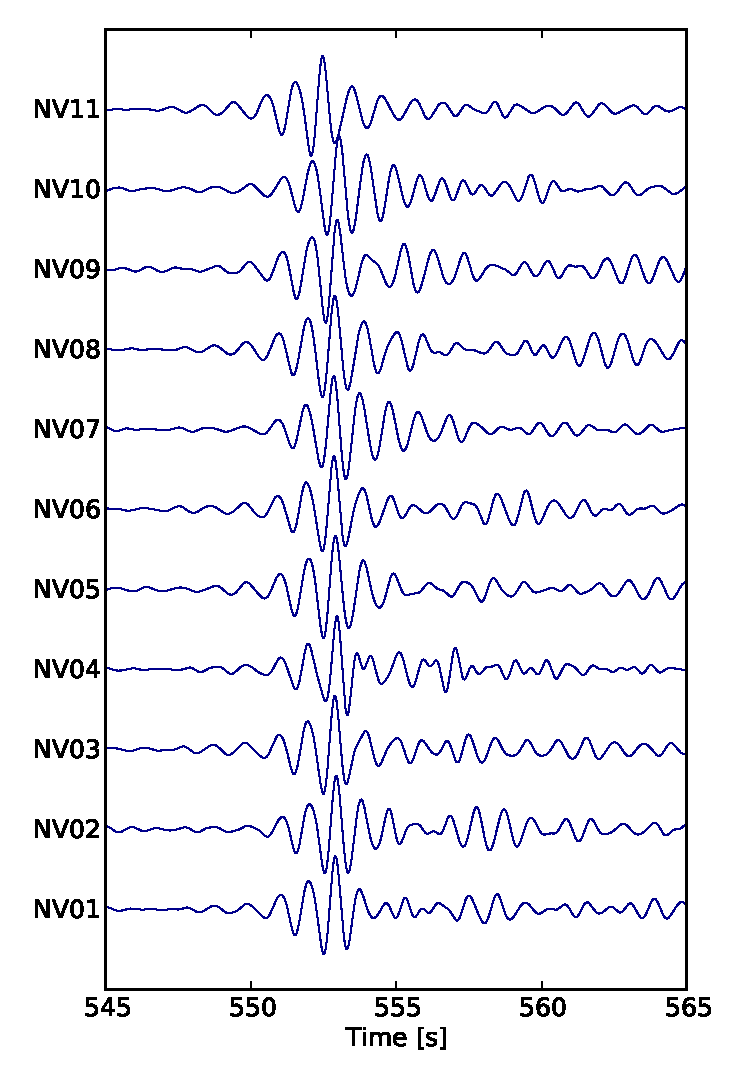
\includegraphics[width=5cm,height=8cm]{fig/chap3/4371355_pcp_sec.eps}
}
	\\
	\subfloat[]{%
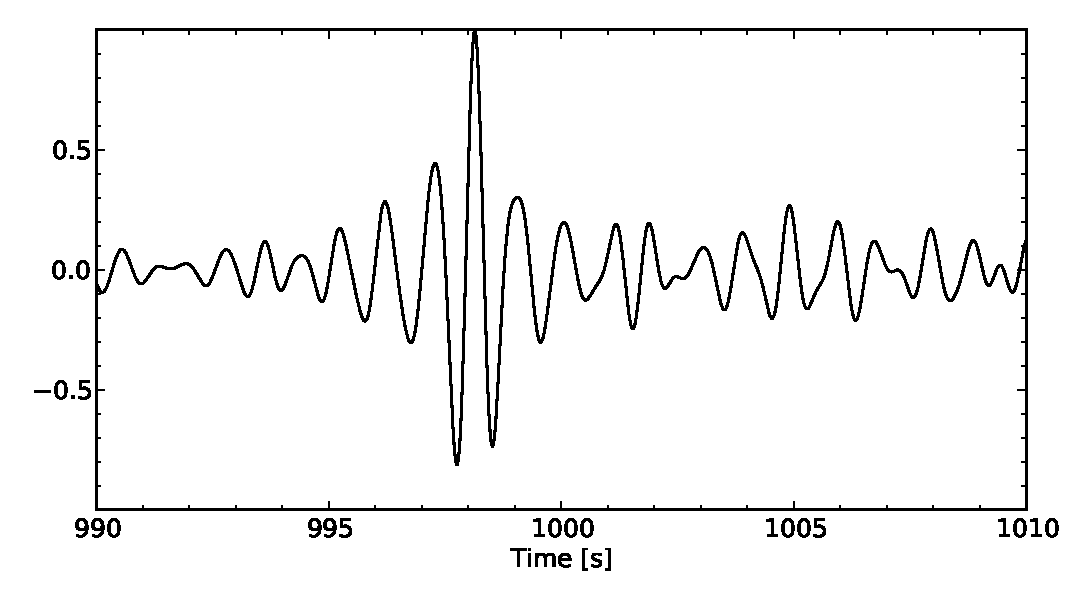
\includegraphics[width=5cm,height=2.5cm]{fig/chap3/4371355_pkikp_stack.eps}
}
	\hspace{3em}
	\subfloat[]{%
\includegraphics[width=5cm,height=3.5cm]{fig/chap3/4371355_nvar_loc.eps}
}
	\caption{(a)NVAR台阵的PKiKP记录(b)PcP所有单道记录(c)线性叠加后的PKiKP波形(d)事件和%
NVAR台阵的位置关系,和地震的震源机制。}
\end{figure}

\newpage

\subsubsection{WRA}

\begin{figure}[!ht]
	\centering
	\subfloat[]{%
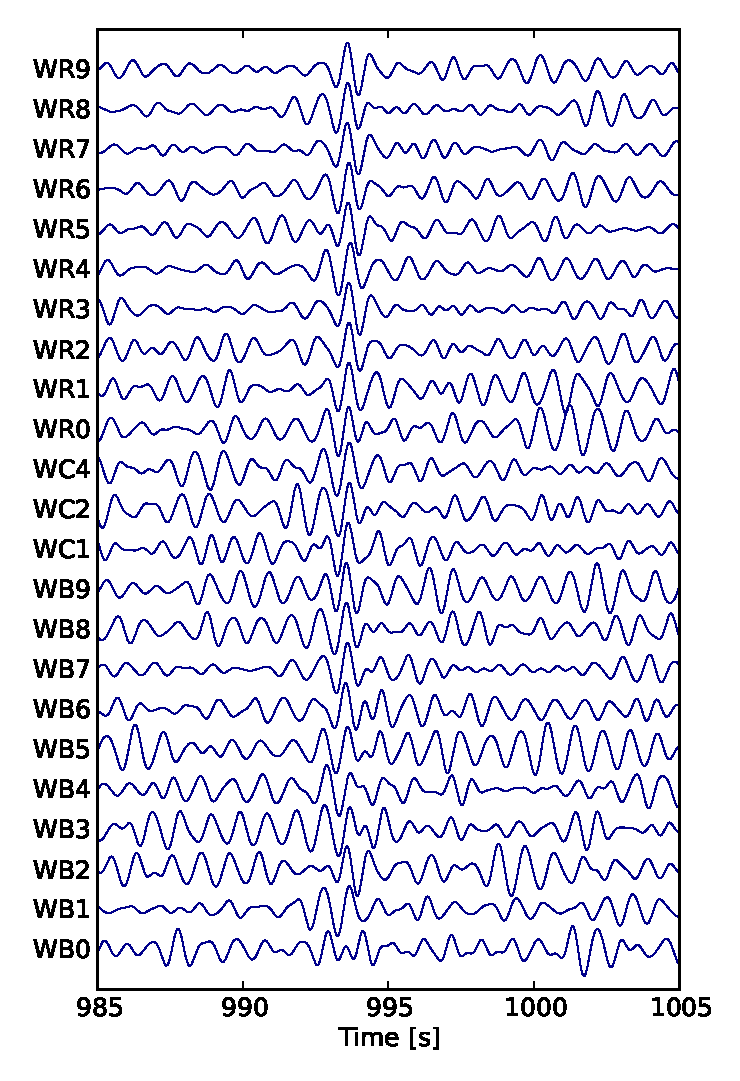
\includegraphics[width=5cm,height=8cm]{fig/chap3/2844731_pkikp_sec.eps}
}
	\hspace{2em}
	\subfloat[]{%
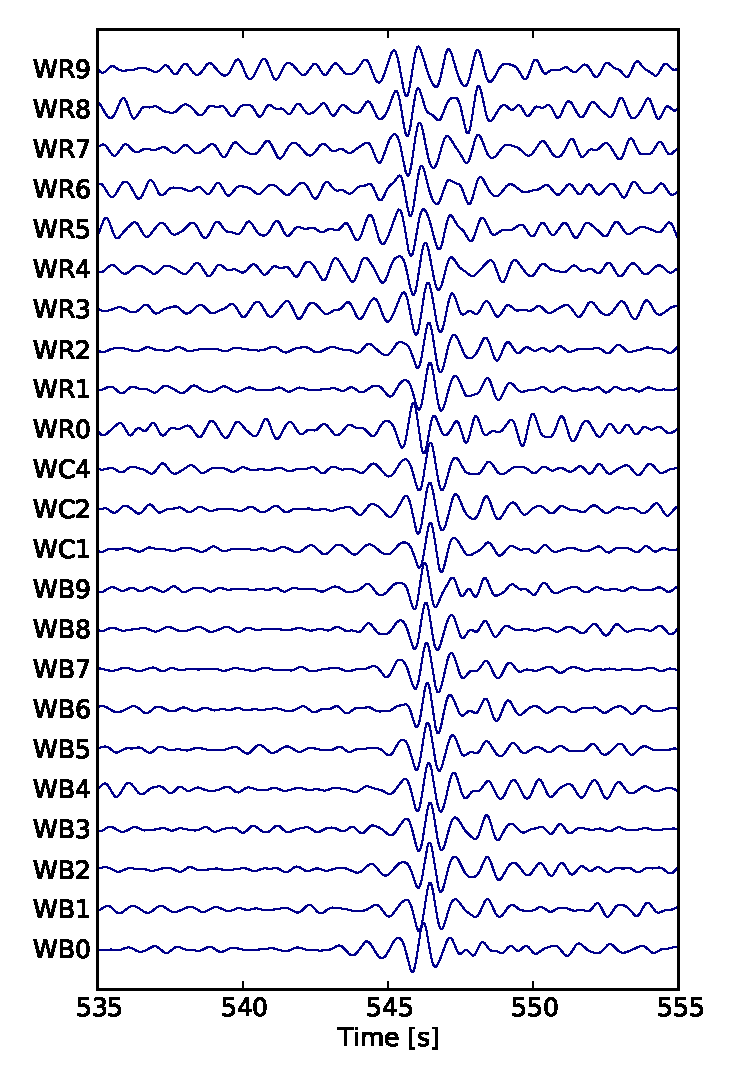
\includegraphics[width=5cm,height=8cm]{fig/chap3/2844731_pcp_sec.eps}
}
	\\
	\subfloat[]{%
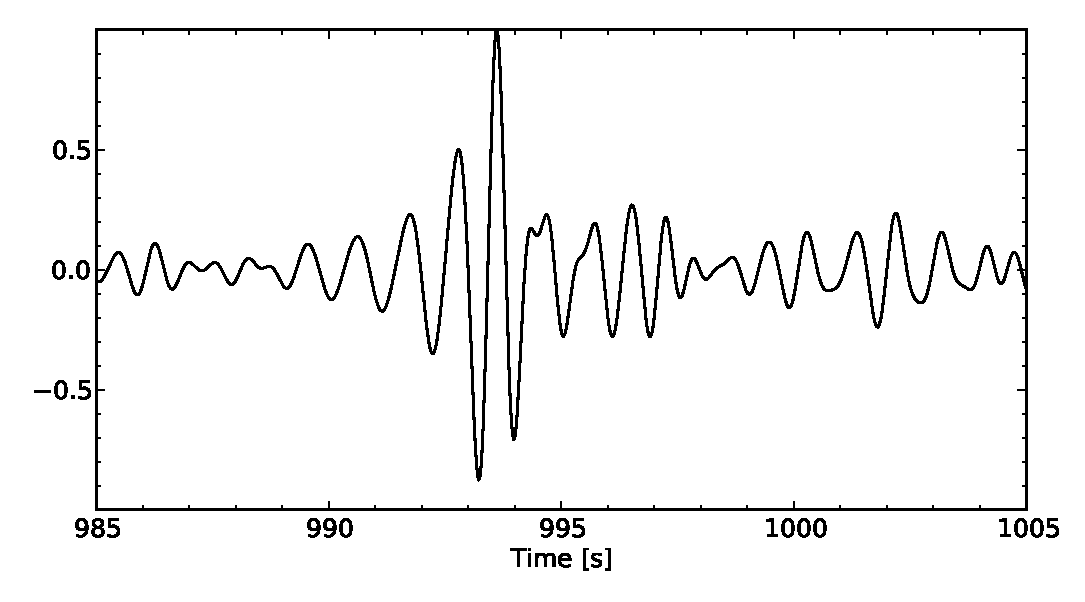
\includegraphics[width=5cm,height=2.5cm]{fig/chap3/2844731_pkikp_stack.eps}
}
	\hspace{3em}
	\subfloat[]{%
\includegraphics[width=5cm,height=3.5cm]{fig/chap3/2844731_wra_loc.eps}
}
	\caption{(a)WRA台阵的PKiKP记录(b)PcP所有单道记录(c)线性叠加后的PKiKP波形(d)事件和%
WRA台阵的位置关系,和地震的震源机制。}
\end{figure}

\newpage

\subsubsection{ABKAR}

\begin{figure}[!ht]
	\centering
	\subfloat[]{%
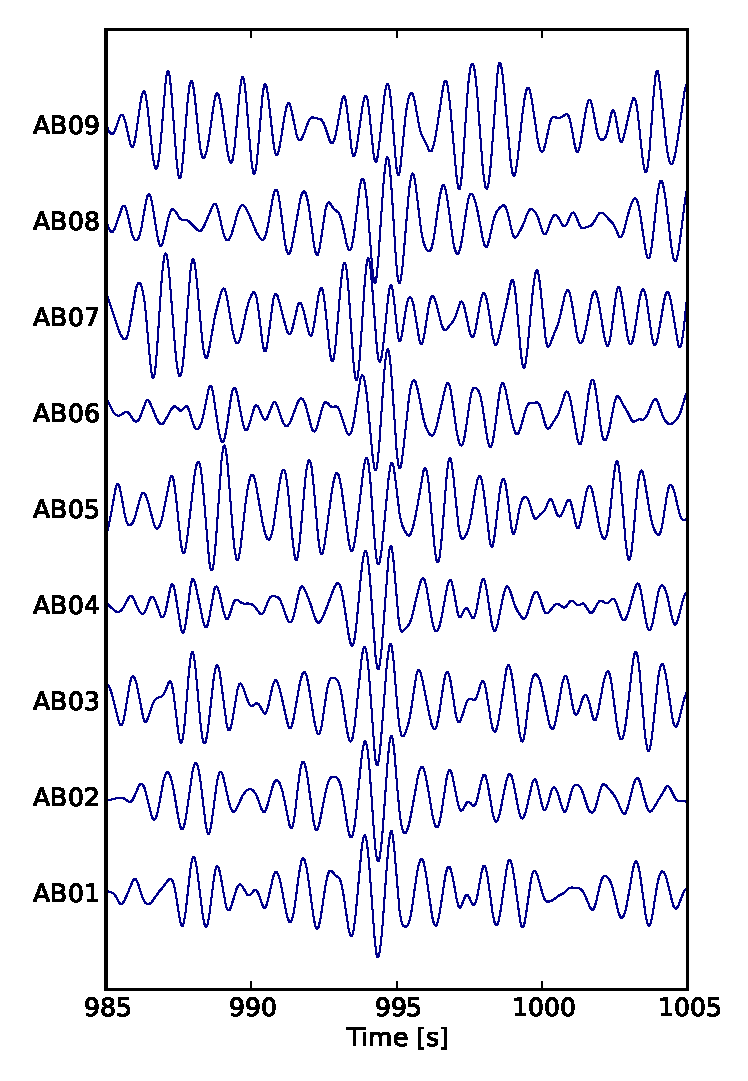
\includegraphics[width=5cm,height=8cm]{fig/chap3/4370774_pkikp_sec.eps}
}
	\hspace{2em}
	\subfloat[]{%
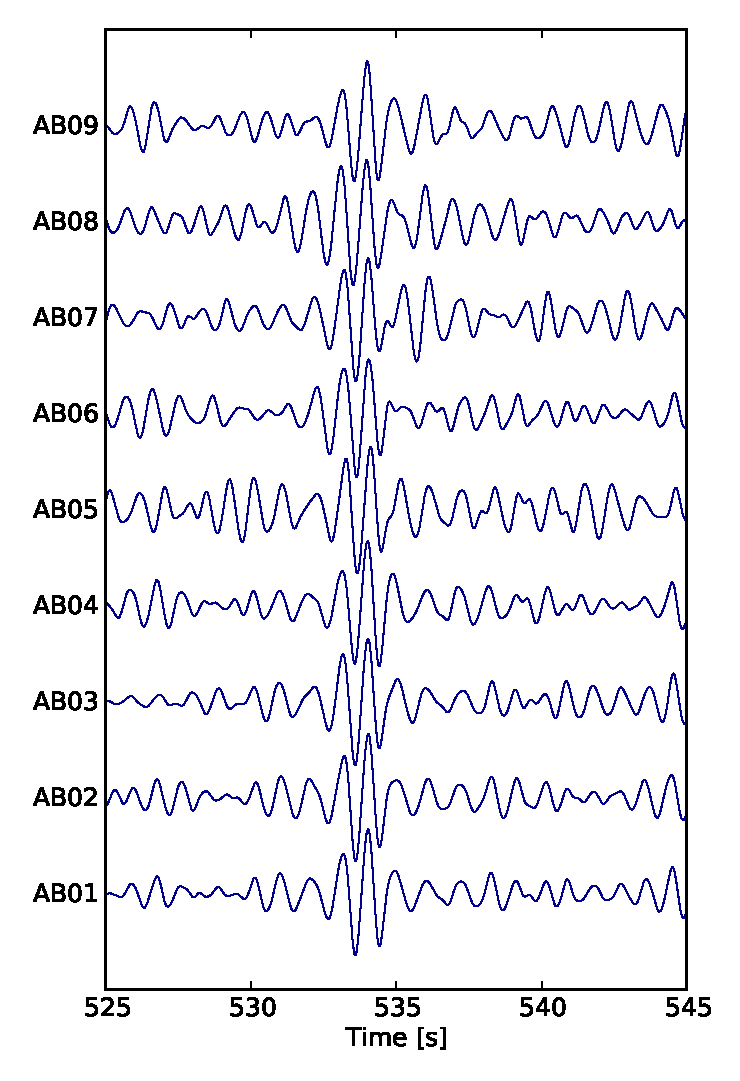
\includegraphics[width=5cm,height=8cm]{fig/chap3/4370774_pcp_sec.eps}
}
	\\
	\subfloat[]{%
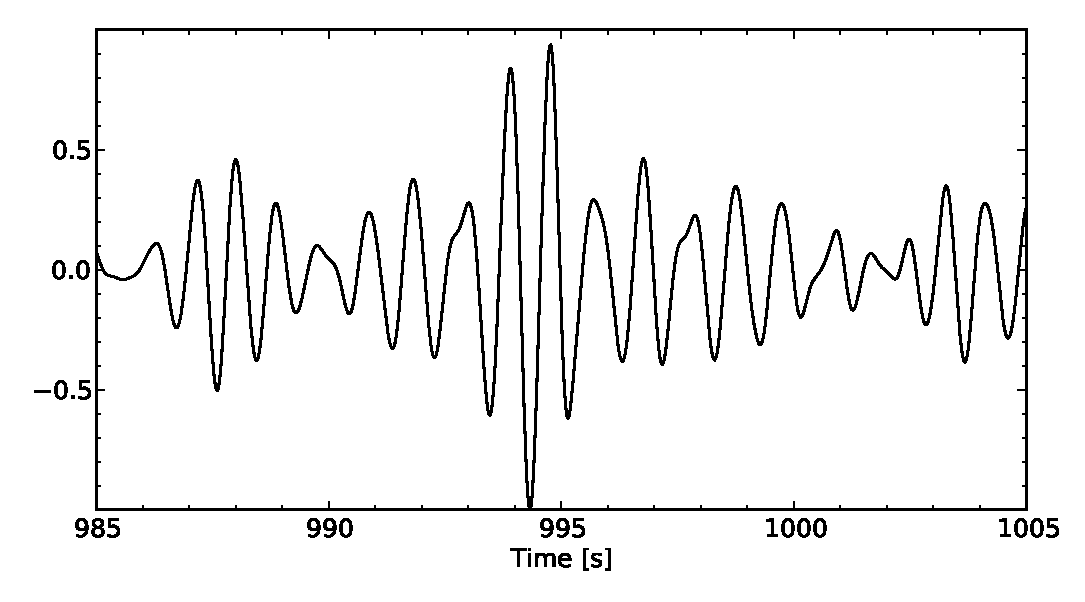
\includegraphics[width=5cm,height=2.5cm]{fig/chap3/4370774_pkikp_stack.eps}
}
	\hspace{3em}
	\subfloat[]{%
\includegraphics[width=5cm,height=3.5cm]{fig/chap3/4370774_abkar_loc.eps}
}
	\caption{(a)ABKAR台阵的PKiKP记录(b)PcP所有单道记录(c)线性叠加后的PKiKP波形(d)事件%
和ABKAR台阵的位置关系,和地震的震源机制。}
\end{figure}

\newpage

\subsubsection{GERES}


\begin{figure}[!ht]
	\centering
	\subfloat[]{%
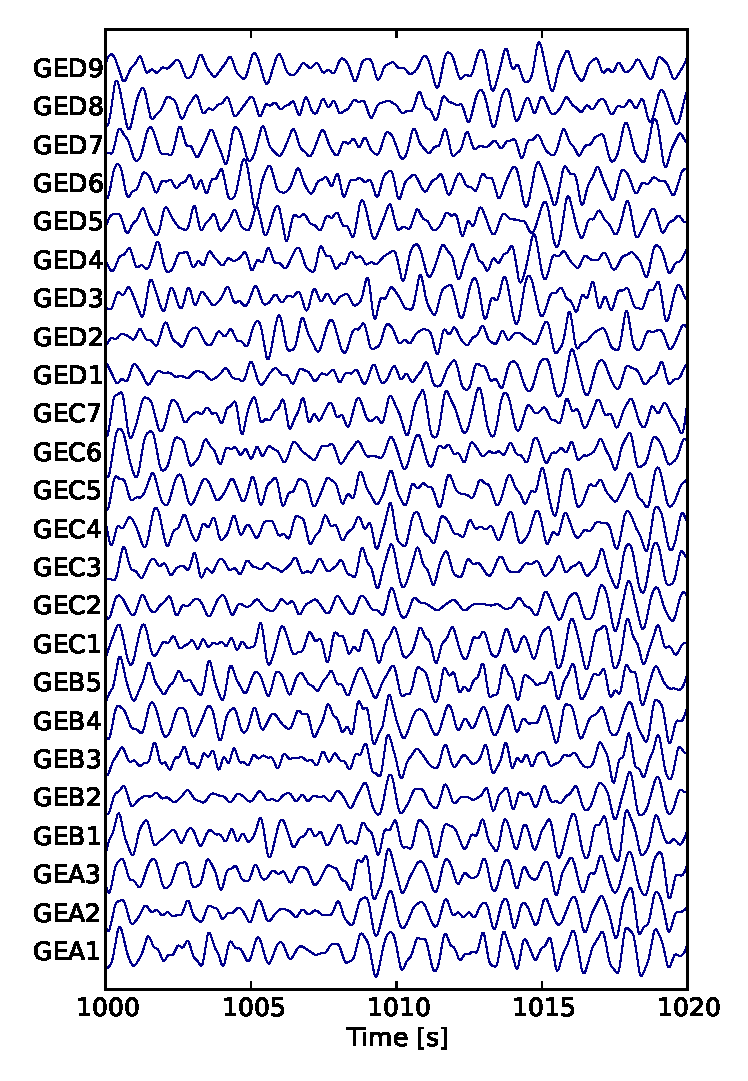
\includegraphics[width=5cm,height=8cm]{fig/chap3/1276871_pkikp_sec.eps}
}
	\hspace{2em}
	\subfloat[]{%
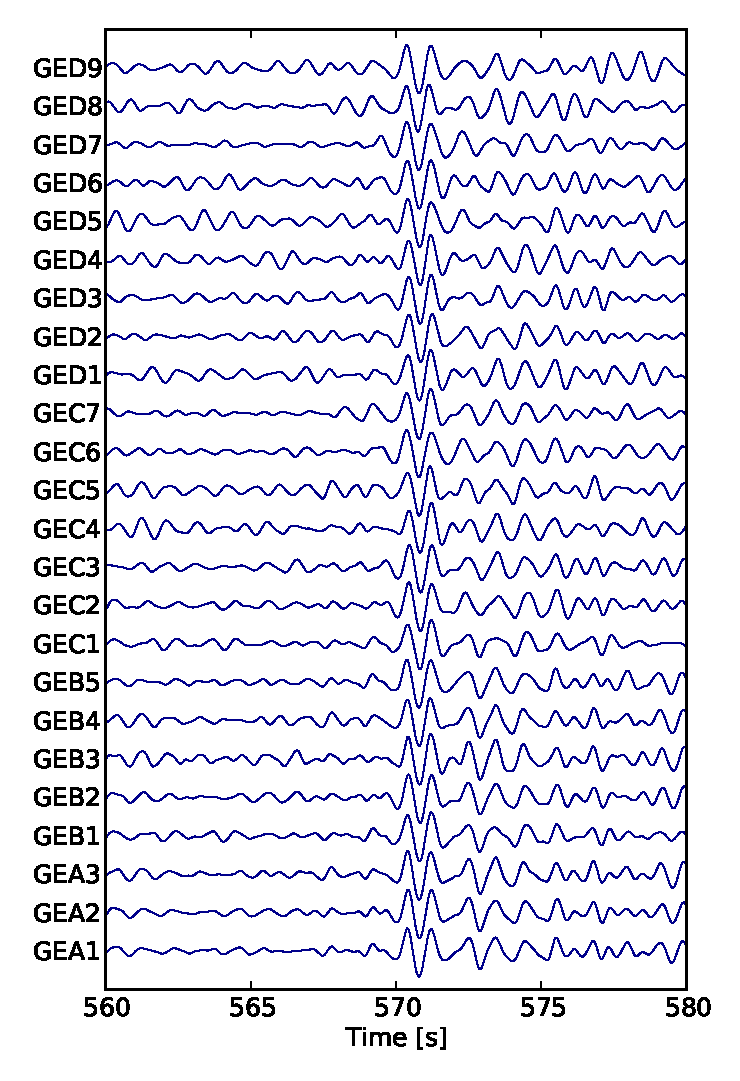
\includegraphics[width=5cm,height=8cm]{fig/chap3/1276871_pcp_sec.eps}
}
	\\
	\subfloat[]{%
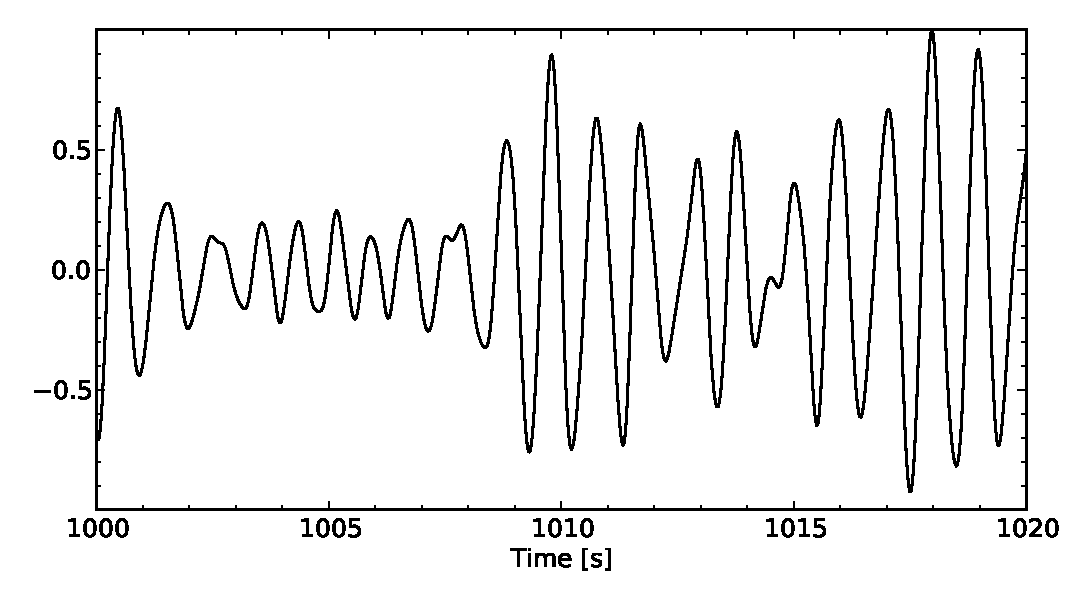
\includegraphics[width=5cm,height=2.5cm]{fig/chap3/1276871_pkikp_stack.eps}
}
	\hspace{3em}
	\subfloat[]{%
\includegraphics[width=5cm,height=3.5cm]{fig/chap3/1276871_geres_loc.eps}
}
	\caption{(a)GERES台阵的PKiKP记录(b)PcP所有单道记录(c)线性叠加后的PKiKP波形(d)事件%
和GERES台阵的位置关系,和地震的震源机制。}
	\label{geres}
\end{figure}

在欧洲大陆台阵观测到的PKiKP振幅均很弱,从图\ref{geres}中德国GERES台站的记录可以看到,虽然具有很清晰的PcP相位,但PKiKP几乎淹没在噪声中,仅仅是根据每道中波形的相似性判断出PKiKP的存在,而且并不是所有的台站都能看到这个信号,在叠加的PKiKP波形之后还存在一段较大振幅的尾波。

\newpage

\subsection{Observations from dense regional networks}

\subsubsection{USArray \& AK}

前面提到,先用IMS台阵快速搜索产生可观测到PKiKP的事件,再用附近的密集台网找到更多的PKiKP的记录,以提升搜索效率。这里给出USArray和阿拉斯加区域台网AK的两个例子。对于USArray,先用NVAR找到2009
年发生在墨西哥的一个地震事件
(2009/04/27 16:46:27,16.95{\textdegree}N/99.57{\textdegree}W,MW 5.8)
然后从当时在运作的378个USArray台站数据中得到了43道清晰的PKiKP观测,如图\ref{usarray_loc}和图\ref{ak_loc},震中距从12度到34度;对与
AK,用BCAR找到的ALEUTIAN群岛的一个事件(2015/01/18 04:47:38, 51.92{\textdegree}N/179.
58{\textdegree}E,MW 5.5),从99个AK台站数据中找到了25道清晰的PKiKP的观测。可见,利用小台阵
和密集台网,前临界PKiKP的寻找并不再那么困难。 

\begin{figure}[!ht]
	\centering
	\includegraphics[width=8cm,height=5cm]{fig/chap3/usarray_loc.eps}
	\caption{对于事件(2009/04/27 %
16:46:27,16.95{\textdegree}N/99.57{\textdegree}W,MW 5.8),观测到PKiKP的USArray的%
台站。其中黑色三角形的代表仅观测到清晰PKiKP的台站,蓝色三角形表示同时观测到清晰PcP和PKiKP%
的台站,绿色的大三角形是用于搜索地震事件的NVAR台阵。红色五角星表示地震位置,旁边标出了其震源%
机制。}
	\label{usarray_loc}
\end{figure}

\begin{figure}[!ht]
	\centering
	\includegraphics[width=8cm,height=5cm]{fig/chap3/ak_loc.eps}
	\caption{对于事件(2015/01/18 04:47:38, 51.92{\textdegree}N/179.%
58{\textdegree}E,MW 5.5),观测到清晰PKiKP的AK台站,图中的标注同图\ref{usarray_loc}。}
	\label{ak_loc}
\end{figure}

从图\ref{usarray_loc}可以看到,就单一事件,PKiKP的观测已经可以覆盖非常大的区域,如果增加更多的事件,利用USArray不同期的台站,所有能找到的PKiKP观测可以将美国下方的ICB覆盖,即可以对此区域的
ICB做整体的分析和研究,从而得到对ICB更全面深刻的认识。

在所有观测到PKiKP的USArray台站中,只有一半同时观测到清晰的PcP和PKiKP,这也暗示了CMB性质随区域可能有强烈的变化,且CMB的性质变化对PKiKP的影响可能不大。同时对于USArray,观测到的PKiKP波形也
很复杂,随着不同台站变化很大,有的台阵上观测到的PKiKP比较尖锐,是一个独立的相位,而有的则看上去是两个分立的相位的部分叠加,有的波形平滑,有的发生了波形的扭曲,这些都体现了PKiKP所经过路径周围的结构对波形的影响,而且在超过20度震中距的情况下,这些影响的产生效应则更加的明显。在这个震中距范围,
PKiKP的理论走时曲线已经有一定弯曲,在较小震中距区间(10\~20),实际PKiKP的波形排列几乎与理论走时曲线平行,且相差大约5秒,但在之后逐渐向前接近理论走时位置。

\begin{figure}[!ht]
	\centering
	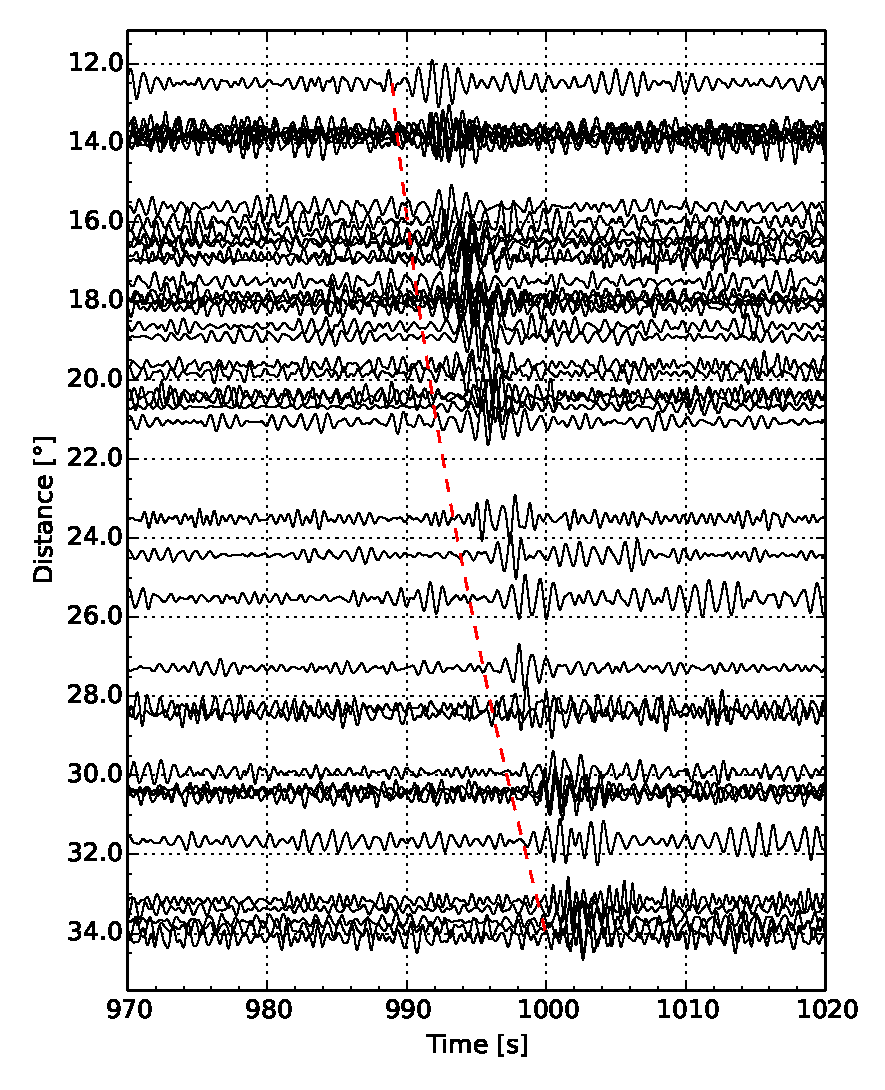
\includegraphics[width=10cm,height=12cm]{fig/chap3/usarray_sec.eps}
	\caption{USArray台网观测到的43道清晰PKiKP波形,震中距从12度到34度,红色虚线表示PREM%
理论PKiKP到时。}
	\label{usarray_sec}
\end{figure}

在北美不同纬度上,观测到的PKiKP实际走时也有明显差异,这可以从USArray和AK台网观测到的PKiKP绝对走时的区别体现出来(图\ref{usarray_sec}、图\ref{ak_sec})。AK台站的PKiKP略提前于PREM理论走时,而USArray的则相对滞后,这个差异可能包含了地球椭率、内核半径和其他结构的贡献。

\begin{figure}[!ht]
	\centering
	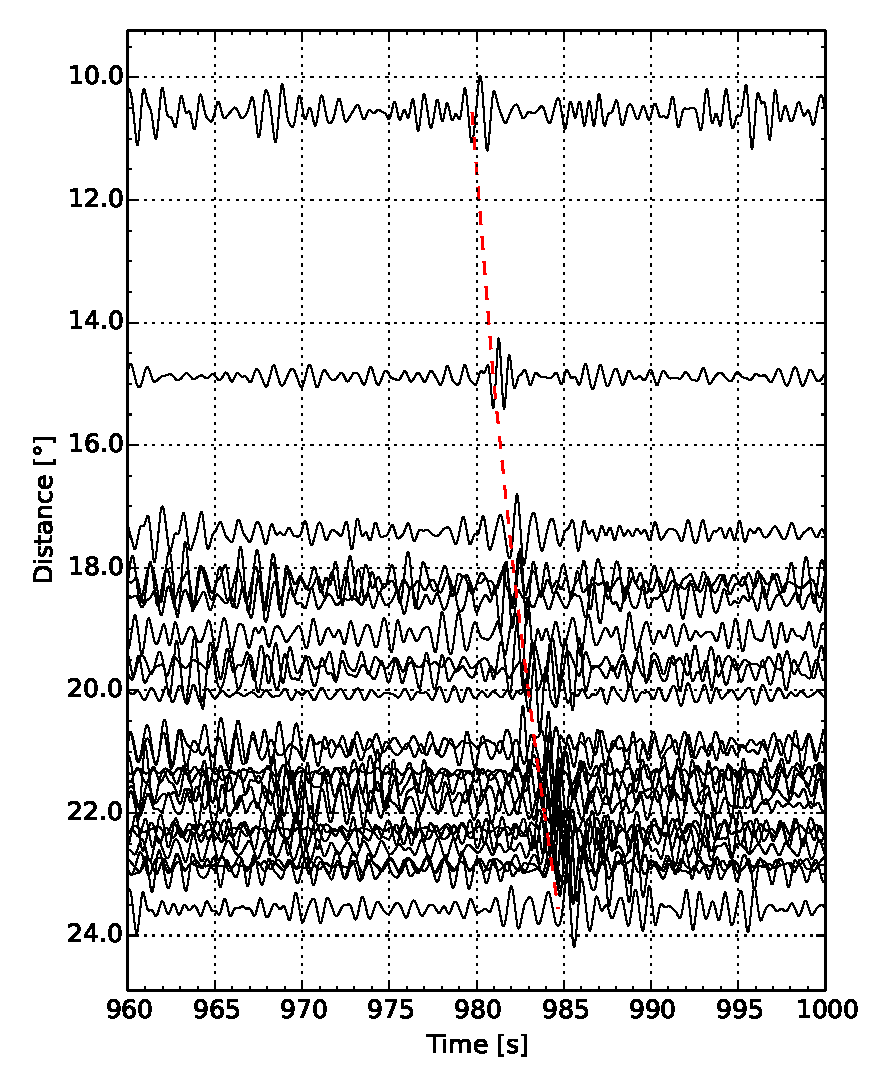
\includegraphics[width=10cm,height=12cm]{fig/chap3/ak_sec.eps}
	\caption{AK台网观测到的43道清晰PKiKP波形,震中距从10度到24度,红色虚线表示PREM%
理论PKiKP到时。}
	\label{ak_sec}
\end{figure}

\newpage

\section{PKiKP Precursor}

\begin{figure}[!ht]
	\centering
	\subfloat[]{%
	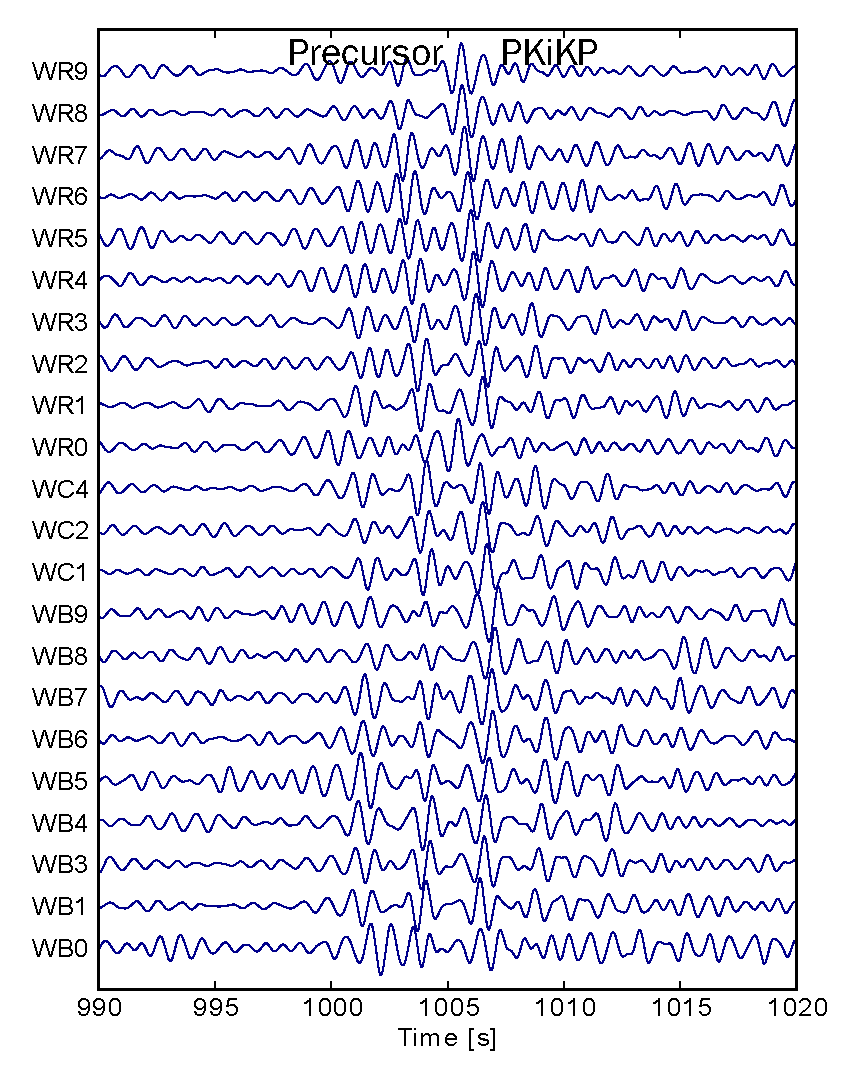
\includegraphics[width=6cm,height=8cm]{fig/chap3/wra_pre_sec.eps}
}
	\hspace{2em}
	\subfloat[]{%
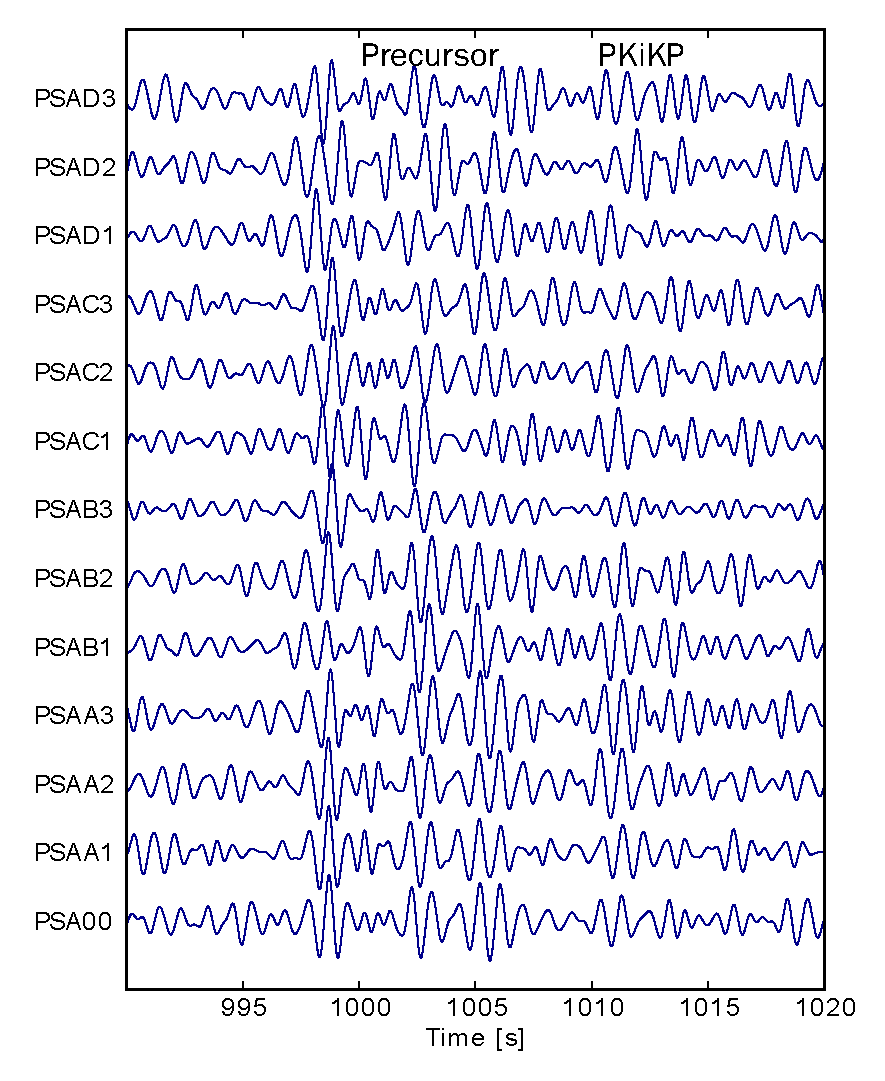
\includegraphics[width=6cm,height=8cm]{fig/chap3/psar_pre_sec.eps}
}	
	\\
	\subfloat[]{%
	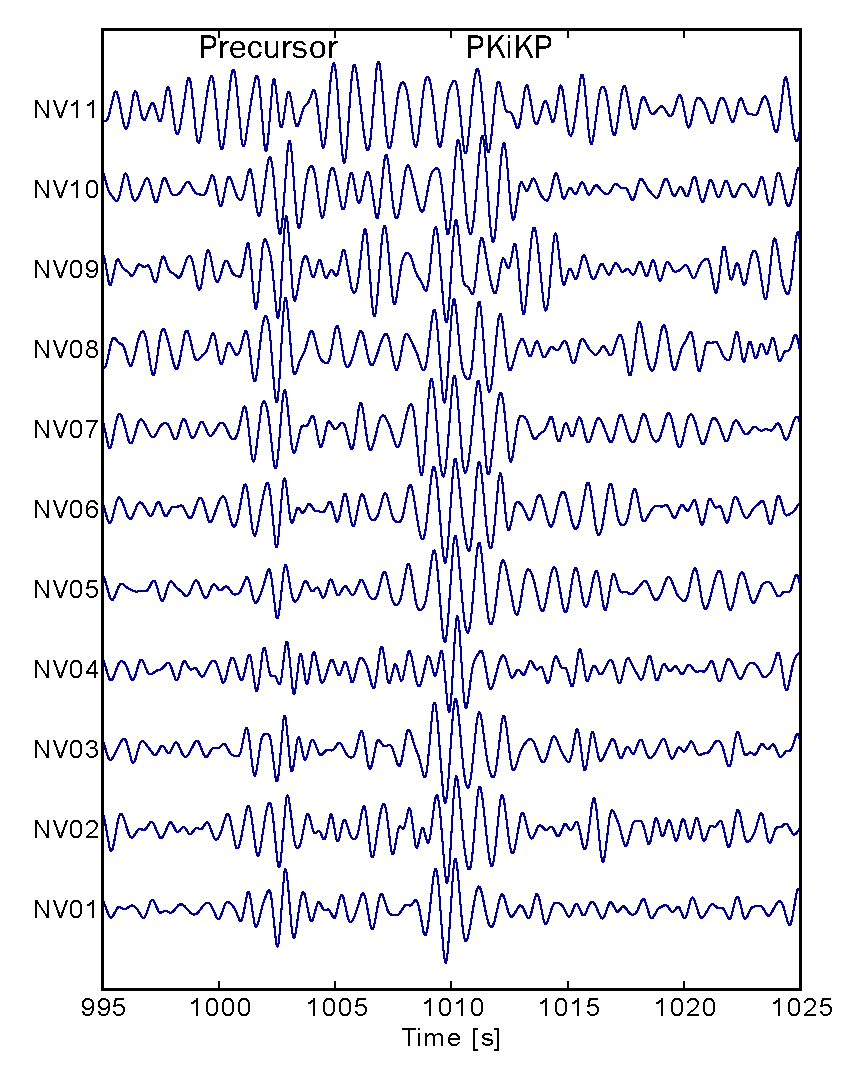
\includegraphics[width=6cm,height=8cm]{fig/chap3/nvar_pre_sec.eps}
}
	\hspace{2em}
	\subfloat[]{%
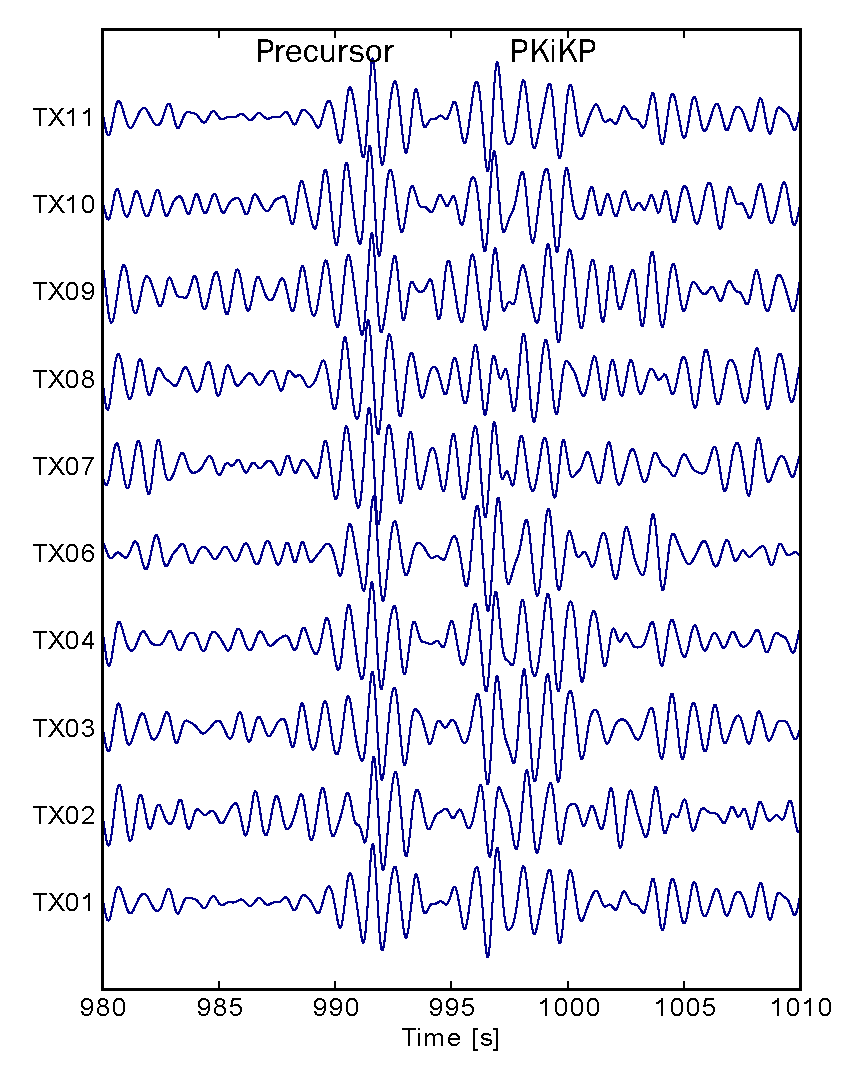
\includegraphics[width=6cm,height=8cm]{fig/chap3/txar_pre_sec.eps}
}
	\caption{PKiKP and its precursor observed in (a)WRA. (b)PSAR. (c)NVAR. (4)%
TXAR.}
	\label{pre}
\end{figure}

在PKiKP到时附近,除了孤立的PKiKP相位,有时在其前数秒观测到Precursor的存在,而且还很清晰如图\ref{pre},可能是来自于某界面的反射震相,但还不知如何解释其来源。

\newpage

\section{PKiKP Coda}


到目前为止的地震学观测表明,内核并不是一个均匀的球体,PKP和PKIKP走时的观测~\citep{Creager1992}和
自由振荡的观测~\citep{Tromp1993}都支持其内部存在各向异性; 由赤道向路径的PKIKP和PKP走时观测也表明内核
存在东西半球的地震波速差异~\citep{Tanaka1997},即内核存在1-Degree尺度的不均匀性。同时内核也被认为存在
强烈的衰减,但目前的研究主要考虑的是内核粘弹性造成的真实衰减,由于内核不均匀的尺度仍不确定,散射衰减对
经过内核的体波总体衰减的贡献也不清楚。之前的研究~\citep{Vidale2000}认为PKiKP的尾波来自外层内核不均匀体
的散射,且散射体的尺度约为2km。后续区域性的~\citep{Poupinet2004}和全球范围的PKiKP尾波研究~\citep{Koper2004}均观测到了持续200s左右的PKiKP尾波,且认为尾波来自于内核的散射。

这里结合全球范围内近十年的数据,对全球范围内观测到的PKiKP尾波进行分析。PKiKP的尾波的可能来源并不唯一,除了内核成因,其也可能来自地幔和地壳的散射。之前的研究通过对比PcP,ScP和PKiKP的尾波的差异来排除尾波地幔成因~\citep{Koper2004},然而即使是小震中距,PcP和PKiKP的路径在地幔中仍有较大的差异,尤其是在下地幔附近,因此为了确定尾波的来源还需要其他区的参照。下面采用的方法是
(1)同一事件不同区域台阵接收到的信号;(2)同一个台阵的PcP,ScP和PKiKP尾波的比较;(3)台阵接收到的发生在同一区域的不同地震的PKiKP波形的比较。

\subsection{Northern America}

2014/06/23 在ALEUTIAN群岛的事件(51.95N 178.58E,Depth 106,MB 6.0),产生的PKiKP相位
同时被位于北美的BCAR,IMAR,BMAR,YKA,NVAR和PDAR等多个IMS台阵接收到,PKiKP采样
位于阿拉斯加附近下方的ICB。图\ref{alas}显示了地震与IMS台阵的位置,以及PKiKP内核反射点的投影。

\begin{figure}[!ht]
	\centering
	\includegraphics[height=6cm,width=10cm]{fig/chap3/ALAS.eps}
	\caption{2014/06/23 22:29:51发生在ALEUTIAN群岛的事件(51.95N 178.58E,Depth 106,MB%  
6.0)和IMS台阵的位置。黑色三角形表示IMS台阵ILAR,BCAR,IMAR,BMAR,YKA,NVAR和PDAR,红色五角星表示地震位置,圆圈表示在ICB反射点的投影,其中绿色表示观测到有PKiKP,黄色表示未观测到PKiKP的台阵ILAR对应的反射点。}
	\label{alas}
\end{figure}

分别对NVAR台阵每道数据进行1-2HZ和2-3HZ频带范围的滤波,可以看出PKiKP的尾波和PKiKP主相位的能量均集中在
1-2HZ内,在2-3HZ范围内滤波后PKiKP被滤掉,每道的振幅为1-2HZ数十分之一(图\ref{nvar_sec}),且紧随着
PKiKP后面的尾波部分的振幅接近前后的噪声级别。在1175s左右似乎存在一个突然出现的能量,而且在提高滤波频率后,
振幅变得更加清晰,这是否是某个特殊的相位还有待确认。

\begin{figure}
\hfill{}
\subfloat[1-2HZ]{%
\centering
\includegraphics[width=6.5cm,height=8.5cm]{fig/chap3/nvar_sec1.eps}
}
\hfill{}
\subfloat[2-3HZ]{%
\centering
\includegraphics[width=6.5cm,height=8.5cm]{fig/chap3/nvar_sec2.eps}
}
\hfill{}
\caption{NVAR台阵记录的ALEUTIAN群岛事件的PKiKP尾波(a)经过1-2HZ滤波的结果(b)经过2-3HZ滤波的结果。}
\label{nvar_sec}
\end{figure}


与之前的研究不同,对于这个事件,NVAR台阵上观测到的PKiKP尾波的持续时间不到100s,而且在PKiKP后续50s内,
存在连续的峰值,振幅可以与PKiKP主相位相当。对PcP,ScP和PKiKP分别进行波包叠加的结果如图\ref{nvar_env},可以看出三者的尾波形态存在明显的差异。PcP的尾波在PcP最大振幅后直接衰减,ScP和PKiKP在主相位后立刻出现一个很大的振幅,但其后ScP尾波逐渐衰减到噪声级别,而PKiKP尾波振幅仍然持续到后80s左右。这说明,PKiKP的尾波与PcP和ScP的可能来源于不同的深部结构。

\begin{figure}
	\centering
	\includegraphics[width=10cm,height=7cm]{fig/chap3/nvar_env.eps}
	\caption{PcP,ScP,PKiKP的尾波波包对比,每道均按照理论的慢度进行叠加,最后再按主相位最大波包振幅%
归一化。}
	\label{nvar_env}
\end{figure}

在这些能观测到清晰PKiKP相位的IMS台阵中,只有在NVAR发现了明显的尾波,且尾波紧随PKiKP主相位,其线性叠加
和PWS叠加的结果见图\ref{nvar_mul};其他台阵上均没有发现类似的现象,PKiKP均较为清晰,且没有续至相位,
见图\ref{others},这很大程度上排除了后续的尾波来自于震源一侧,例如在震源侧反射的深度相位
;对于没有观测到PKiKP相位的台阵ILAR,在PKiKP理论到时后也没有大于噪声级别的振幅。在叠加
的PDAR台阵的PKiKP波形中,大约在主PKiKP相位后5s出现一个续至相位的振幅,这与叠加的NVAR台阵波形一致。由于
PDAR和NVAR相距较近,且相对与事件的震中距都在45\textdegree左右,这个相位可能是来源与地壳,但NVAR后续
的应该来自于更深的地方。在震中距为60\textdegree的TXAR台阵,既没有观测到直达的PKiKP相位也没有观测到任何
尾波存在的迹象。值得注意的是NVAR,PDAR和TXAR有较为接近的方位角,分别为81.4\textdegree,71.2\textdegree和79.6\textdegree。

\begin{figure}
	\centering
	\includegraphics[width=12cm,height=6cm]{fig/chap3/nvar_mul.eps}
	\caption{NVAR台阵对2014/06/13事件的PKiKP及其尾波的叠加结果,均根据理论慢度进行叠加。上部为波包%
叠加(与图\ref{nvar_env}中的相同),中为相加权叠加(PWS),下为线性叠加,均能看到清晰的PKiKP和其后续的尾波。}
	\label{nvar_mul}
\end{figure}


\begin{figure}[tbph]
\centering
\subfloat[IMAR]{%
\centering
\includegraphics[width=6cm,height=4cm]{fig/chap3/imar_mul.eps}
}
\hspace{2em}
\subfloat[BCAR]{%
\centering
\includegraphics[width=6cm,height=4cm]{fig/chap3/bcar_mul.eps}
}\\
\subfloat[YKA]{%
\centering
\includegraphics[width=6cm,height=4cm]{fig/chap3/yka_mul.eps}
}
\hspace{2em}
\subfloat[PDAR]{%
\centering
\includegraphics[width=6cm,height=4cm]{fig/chap3/pdar_mul.eps}
}
\caption{IMAR,BCAR,YKA,PDAR台阵观测到的PKiKP相位,上为波包叠加,中为PWS叠加,下为线性叠加。%
震中距分别为,19.7\textdegree,23.5\textdegree,36.0\textdegree,47.7\textdegree。}
\label{others}
\end{figure}

令人感到疑惑的是,一小时前在该事件发生处附近的另一个事件(21:11:40,51.95N 178.45E)
深度103km,震级与后者相同,但NVAR并没有记录到与该事件类似的PKiKP尾波(图\ref{nvar_mul2})。

\begin{figure}
	\centering
	\includegraphics[width=12cm,height=6cm]{fig/chap3/nvar_mul2.eps}
	\caption{NVAR台阵对2014/06/23前一个事件的PKiKP及其尾波的叠加结果,均根据理论慢度进行叠加。%
上部为波包叠加,中为相加权叠加(PWS),下为线性叠加,可以看见明显的PKiKP,但没有明显的尾波。}
	\label{nvar_mul2}
\end{figure}

\subsection{Australia}

本文的尾波分析在澳大利亚一共用到了三个小口径台阵的数据,分别是WRA、ASAR和PSAR,它们在之前的研究中也被用到,这里增加了一个螺旋形的PSAR台阵。在这些台阵上观测到的PKiKP尾波和之前研究的有相同的特征(\ref{asar_mul}),包括长的持续时间和平滑的衰减,但并不没有之前研究所提到那么高频,进行1-2HZ的滤波后PKiKP的尾波已经具有足够大的能量,但当滤波频率提高到2-3HZ,尾波振幅则大大减小,所以1-2HZ是比较适合观测这个区域尾波的频率范围。观测到尾波的事件位置如图\ref{au_coda},可以发现这其中有很多地震的位置与之前研究中观测到尾波的事件处于同一区域,而这里使用的是完全不同时期的数据,这说明PKiKP尾波的观测是可靠的。

\begin{figure}
	\centering
	\includegraphics[width=10cm,height=8cm]{fig/chap3/AU_coda.eps}
	\caption{位于Australia的IMS台阵观测到尾波的事件,红色五角星表示地震,连接事件和台%
阵的黑色线表示射线路径的投影,黑色三角形表示台阵,台阵名在其旁边的方框中标出。}
	\label{au_coda}
\end{figure}

\begin{figure}
	\centering
	\includegraphics[width=12cm,height=6cm]{fig/chap3/asar_mul.eps}
	\caption{ASAR台阵对表中事件的PKiKP波形及其叠加结果,均根据理论慢度进行叠加。%
上部为单道波形,下为相加权叠加(PWS),中为线性叠加,可以在单道上看到很大的PKiKP尾波能量。}
	\label{asar_mul}
\end{figure}

为了确认PKiKP之后的信号确实是尾波,而非单个事件在某个台阵的产生的偶然结果,这里将ASAR台阵接收到的4个地震
事件的PKiKP附近的波形进行比较,发现均出现相似的尾波,这4个地震位置相差不到1度,且震源深度也很接近,
见表\ref{evtlst1}。由此可以推测,这可能是来自深部同一源产生的散射能量。同时可以发现,第四个事件产生的PKiKP尾波振幅较小,可能是其震级较前三个事件小(MW 5.7),激发的散射能量更小的缘故。

\begin{table}[!ht]
\centering
\begin{tabular}{*{3}{l}*{2}{c}*{2}{l}}
\hline
n & Date & Hour & Latitude & Longitude & Depth & Magnitude\\
\hline
1 & 2012/07/28 & 20:03:56.8 &  -4.651  &  153.173  &  41  & 6.5\\
2 & 2012/08/02 & 09:56:41.7 &  -4.654  &  153.275  &  46  & 6.1\\
3 & 2012/12/15 & 19:30:02.1 &  -4.632  &  153.016  &  52  & 6.1\\
4 & 2012/07/07 & 03:35:28.5 &  -4.651  &  153.296  &  35  & 5.7\\
\hline
\end{tabular}
\caption{四个位置相近的地震的震源参数。}
\label{evtlst1}
\end{table}

\begin{figure}[tbph]
	\centering
	\includegraphics[width=6cm,height=4cm]{fig/chap3/3344573_coda.eps}
	\hspace{2em}
	\includegraphics[width=6cm,height=4cm]{fig/chap3/3347700_coda.eps}\\
	\includegraphics[width=6cm,height=4cm]{fig/chap3/3712078_coda.eps}
	\hspace{2em}
	\includegraphics[width=6cm,height=4cm]{fig/chap3/3343509_coda.eps}
	\caption{4个位置接近的地震在ARSR台阵上产生的PKiKP波包叠加,频率范围为1-2HZ,它们的尾波均持续超过%
100s,图中振幅均为对数坐标。注意到第四个事件的PKiKP尾波振幅较前三个小。}
\end{figure}

之前的研究认为~\citep{Koper2004,Poupinet2004},PKiKP尾波是由之前震相的尾波,例如P,ScP的尾波与由深部散射产生的尾波叠加而成,如果拟合PKiKP到时前的波包趋势,将其向后延伸,如果其延伸之后的
曲线振幅级别小于PKiKP的尾波振幅,可以说明PKiKP之后确实有其他的能量到达台阵,其中有一部分可能是
来自内核不均匀体的散射。从ASAR台阵数据的波包叠加明显反映出这种特征。

\subsection{Asia}

位于哈萨克斯坦的IMS台阵KKAR上也观测到了PKiKP理论到时后的尾波,在记录中没有看到直达的PKiKP震
相,且从叠加的尾波波包来看,尾波大约持续100s左右,且其振幅先经历一段时期的上升,再逐渐减弱。
如图\ref{kkar_coda}。这种特征类似于~\cite{Vidale2000}的观测。

\begin{figure}[!ht]
	\centering
	\includegraphics[width=12cm,height=6cm]{fig/chap3/kkar_sec.eps}
	\caption{KKAR台阵上观测到的尾波。红色的圆圈表示每道的PKiKP到时位置。}
	\label{kkar_coda}
\end{figure}

对于在2013年所有震中距在10{\textdegree}到70{\textdegree}的5级以上地震,这三个IMS台阵仅仅观测到这一个事件产生的明显PKiKP尾波。该事件位于位于北苏门答腊(5.42N/92.82E,depth 15.6km,MW 5.5),震中距42.4{\textdegree},ICB的反射点位于~\cite{Tanaka1997}所划定的东半球。从PWS和线性叠加的结果看来,每道PKiKP尾波并不存在明显的相关性,叠加后的振幅与前后的噪声级别
相当。

\begin{figure}[!ht]
	\centering
	\includegraphics[width=12cm,height=6cm]{fig/chap3/kkar_mul.eps}
	\caption{KKAR台阵的PKiKP尾波叠加结果,均按照理论PKiKP慢度进行叠加。上为波包叠加,中%
间是PWS叠加,下为线性叠加。可以看到叠加的PKiKP尾波波包振幅先增大后衰减的变化。}
\end{figure}

\subsection{Conclusion about PKiKP coda observation}




\chapter{PKiKP/PcP Amplitude Ratio and CMB variation}

利用PKiKP和PcP相位的振幅比可以约束ICB的密度变化和剪切波速度差等性质~\citep{Koper2004a},即
认为PcP和PKiKP在地幔中的射线路径比较接近,则地幔对振幅观测的影响效应可以大部分被消除,同时也可以
避免由于仪器造成的绝对振幅测量不准确的影响,对振幅比异常的贡献主要来自与内核。但这其中隐含了使用
幅比方法研究ICB的一个重要的假设,即核幔边界的性质和结构能比较好的确定且其变化对PKiKP/PcP的振幅
比不敏感。否则,可能会观测到异常大或异常小的PKiKP和PcP振幅比,这样就很难对ICB的性质进行约束。

通过对265对观测到PKiKP相位的事件和台阵对数据的挑选,得到了这两个相位能同时被观测到的111对事件和
IMS台阵的数据,在这个数据集中,两个相位的最大振幅都能较为可靠地被测量。同时,为了探求是什么因素影响
PKiKP和PcP是否同时被观测到,对地震震源参数、震中距和PcP在CMB的反射点位置分布做了一些分析(图
\ref{dep_mag_hist}、图\ref{dis_hist})。从结果来看,对于已有的全部数据,不管是地震的震级、
震源深度还是震中距都不会对这两个相位是否被同时观测到产生太大影响。5.0级之上的事件都可产生清晰
的PcP和PKiKP,这些事件基本集中在0-100km的浅源深度,这也说明在最初对事件的选择不加太多限制是
正确的,较多的5级浅源地震保证了有效数据的数量。

\begin{figure}[!ht]
	\centering
	\includegraphics[width=12cm,height=9cm]{fig/chap4/depmag_hist.eps}
	\caption{(a),(b)分别为观测到PKiKP相位的事件和同时观测到PcP和PKiKP的事件随震源深度%
的分布;(c),(d)分别为观测到PKiKP相位的事件和同时观测到PcP和PKiKP的事件随震级的分布。}
	\label{dep_mag_hist}
\end{figure}

\begin{figure}[!ht]
	\centering
	\includegraphics[width=12cm,height=4.5cm]{fig/chap4/dist_hist.eps}
	\caption{(a),(b)分别为观测到PKiKP相位的事件和同时观测到PcP和PKiKP的事件随震中距%
的分布。}
	\label{dis_hist}
\end{figure}

由于震源深度并不对PKiKP和PcP的可观测性产生较大影响,因此可以很大程度上排除未观测到PcP但观测到
PKiKP是上地幔结构的影响,比如上地幔低速带对PcP振幅的衰减作用。这就更加强烈的暗示了核慢边界的性质
是影响PcP相位观测的主要因素,也说明了CMB结构对PKiKP/PcP振幅比也可能产生巨大影响。从观测和
未观测到的PcP在CMB反射点的分布来看(图\ref{loc_distri}),即使在某个区域内,CMB的性质也可能发生强烈变化(即图中蓝色和红色的交替出现)。

\begin{figure}[!ht]
	\centering
	\includegraphics[width=12cm,height=4cm]{fig/chap4/loc_distri.eps}
	\caption{左图为地震事件的分布,红色五角星表示同时观测到PKiKP和PcP的事件,蓝色五角星表示%
仅观测到PKiKP的事件;右图为PcP在CMB的上的反射点分布,红色圆圈表示同时观测到PKiKP和PcP,蓝色%
圆圈表示仅观测到PKiKP的反射点。}
	\label{loc_distri}
\end{figure}

\section{Local intensive variation of CMB property}

之前的观测已经表明CMB的横向变化会产生异常大的PKiKP/PcP振幅比~\citep{Koper2004a},且是理论预
期的振幅比的数倍。产生异常大的振幅比是因为PcP的振幅异常小,即在由CMB反射式PcP的振幅受到很大的损
失。可能的解释有(1)下地幔底部存在超低速带;(2)核幔边界存在厚的转换带~\citep{Garnero2000}。当
转换带的厚度接近入射波的波长的时候,反射系数会剧烈减小~\citep{richards1972};(3)核慢边界的地
形起伏。地形起伏产生的聚焦和散焦效应会产生异常的PcP振幅~\citep{Neuberg1991}。很难用只用这三
种解释中的一种来解释与理论振幅比相差达到十倍的观测数据,因此异常的PcP振幅很可能是多种因素的共同
的结果。图\ref{nvar_ratio_cor}和图\ref{pdar_ratio_cor}显示了NVAR台阵和PDAR台阵观测的PK
iKP/PcP振幅比分别与PcP、PKiKP振幅的关系。NVAR台阵数据中,PKiKP/PcP震幅比和PcP的振幅显示出强
烈的负相关,而与PKiKP振幅则没有明显关系,表明在NVAR数据采样到的CMB区域可能存在强烈的横向变化;而
对于PDAR台阵,振幅比与PcP的相关性则略小,但振幅比则普遍较NVAR台阵偏高,可能在这部分数据采样的CMB
性质横向变化较弱,且采样区域可能位于低速带中。

\begin{figure}[!ht]
	\centering
	\includegraphics[width=12cm,height=4.5cm]{fig/chap4/nvar_ratio_cor.eps}
	\caption{NVAR台阵观测到的PKiKP/PcP振幅比和PcP振幅的关系,其中PcP的振幅用对数坐标表%
示。}
	\label{nvar_ratio_cor}
\end{figure}

\begin{figure}[!ht]
	\centering
	\includegraphics[width=12cm,height=4.5cm]{fig/chap4/pdar_ratio_cor.eps}
	\caption{PDAR台阵观测到的PKiKP/PcP振幅比和PcP振幅的关系,其中PcP的振幅用对数坐标表%
示。}
	\label{pdar_ratio_cor}
\end{figure}

\subsection{Varify CMB effects on Amplitude Ratio}

在111对同时观测到较清晰的PcP和PKiKP的事件-台阵数据集中,有22个地震事件被一个以上的IMS台阵记录
到,这就为检验核慢边界横向变化对PKiKP/PcP振幅比的影响提供了绝佳的条件。还是以NVAR和PDAR两个台
阵为例,在22个事件中由这两个台阵同时观测到的就有10个,震中距都在25{\textdegree}以上,且其中
7个都在31-34{\textdegree}之间,这些事件全都来自墨西哥—危地马拉的地震带,震源位置都比较接近,
震源深度的差别也不是很大。这十个事件见表\ref{nvpd}。通过对比可以发现,不同台阵观测到的PKiKP/Pc
P振幅比可以有巨大的差别,对有的事件NVAR和PDAR两个台阵观测到的振幅比差别竟然能达到10倍之多,而且
在后面的讨论中可以看出这绝不是偶然的情况,如此大的差别很难想象是由除CMB横向变化之外的其他因素所
造成,因为两个台阵到事件的震中距差别不大,NVAR和PDAR也只相距1000公里,同一事件在内核的反射点在内
核表面的距离也小于它们对应于CMB反射点的距离;对某些事件,两个台阵的观测的振幅比则极为接近,可能这
部分事件的数据采样到CMB性质相近的区域。

\begin{table}[!ht]
	\centering
	\begin{tabular}{*{3}{l}*{2}{c}*{2}{l}}
	\hline
	n & Date & Hour & Latitude & Longitude & Depth & Magnitude\\
	\hline
1 & 2003/08/25 & 06:28:34.9 &  13.9932 &  -91.1255 &  99.5 & 5.9\\
2 & 2007/07/23 & 22:30:09.2 &  14.465  &  -90.906  &  115  & 5.5\\
3 & 2009/11/26 & 19:08:10.4 &  13.4767 &  -89.9617 &  48.5 & 5.9\\
4 & 2009/04/27 & 16:46:27.5 &  16.9557 &  -99.5717 &  31.7 & 5.8\\
5 & 2009/05/03 & 16:21:46.4 &  14.6199 &  -91.2025 &  113.9 & 6.3\\
6 & 2009/08/15 & 13:22:43.1 &  18.0998 & -100.6157 &  61.2 & 5.5\\
7 & 2012/06/27 & 06:30:59.8 &  13.834  &  -89.967  &  132.6 & 5.7\\
8 & 2012/11/15 & 09:20:21.9 &  18.346  & -100.382  &  53  & 6.1\\
9 & 2013/07/08 & 02:52:42.6 &  13.2316 &  -89.1292 &  55  & 5.7\\
10 & 2014/01/11 & 13:10:51.1 &  14.6437 &  -92.0592 &  78  & 5.5\\
	\hline
\end{tabular}
	\caption{同时观测到PKiKP和PcP的事件—台阵对数据中同时被NVAR和PDAR台阵观测到的10个事件%
。}
	\label{nvpd}
\end{table}
%\chapter{叠加理论波形}

\backmatter

\bibliographystyle{apalike}
%\bibliography{innercore,noise,array,method,cmb}
\bibliography{seis}
\end{document}